% !TEX program = xelatex
% Laporan Tugas Besar 2 IF3170 Inteligensi Artifisial 2026/2027
% Kelompok 09 - Aduhmen
% Kompilasi di Overleaf: pilih Compiler = XeLaTeX

\documentclass[11pt,a4paper]{article}

% =====================================================================
% PACKAGES & FONTS (IBM Plex Sans 11pt + Courier New 9pt)
% =====================================================================
\usepackage[a4paper,top=3.0cm,bottom=2.5cm,left=2.5cm,right=2.5cm,headheight=42pt,headsep=26pt,footskip=24pt]{geometry}
\usepackage{fontspec}
\IfFontExistsTF{IBM Plex Sans}{
  \setmainfont{IBM Plex Sans}
  \setsansfont{IBM Plex Sans}
}{
  \usepackage[sfdefault]{plex-sans}
}
\renewcommand{\familydefault}{\sfdefault}
\IfFontExistsTF{Courier New}{
  \setmonofont{Courier New}[Scale=0.86]
}{
  \IfFontExistsTF{TeX Gyre Cursor}{
    \setmonofont{TeX Gyre Cursor}[Scale=0.86]
  }{
    \setmonofont{DejaVu Sans Mono}[Scale=0.82]
  }
}

\usepackage[indonesian]{babel}
\usepackage[none]{hyphenat}
\usepackage{graphicx}
\usepackage{amsmath,amssymb}
\usepackage{array}
\usepackage{tabularx}
\usepackage[table]{xcolor}
\usepackage{fancyhdr}
\usepackage{titlesec}
\usepackage{tocloft}
\usepackage{caption}
\usepackage{listings}
\usepackage{float}
\usepackage{enumitem}
\usepackage{setspace}
\usepackage{xurl}
\usepackage[hidelinks]{hyperref}

% =====================================================================
% COLORS & TYPOGRAPHY
% =====================================================================
\definecolor{tblblue}{gray}{0.92}
\definecolor{headergray}{HTML}{555555}
\definecolor{rulegray}{HTML}{888888}

\setstretch{1.15}
\setlength{\parindent}{0pt}
\setlength{\parskip}{6pt}
\emergencystretch=3em
\sloppy

% Heading Sizes: H1 = 16pt, H2 = 12pt, H3 = 11pt
\titleformat{\section}{\fontsize{16}{20}\selectfont\bfseries}{\thesection.}{0.6em}{}
\titlespacing*{\section}{0pt}{14pt}{6pt}

\titleformat{\subsection}{\fontsize{12}{15}\selectfont\bfseries}{\thesubsection.}{0.6em}{}
\titlespacing*{\subsection}{0pt}{11pt}{4pt}

\titleformat{\subsubsection}{\fontsize{11}{14}\selectfont\bfseries}{\thesubsubsection.}{0.6em}{}
\titlespacing*{\subsubsection}{0pt}{9pt}{3pt}

% Caption Style (8pt, bold label)
\DeclareCaptionFont{cap8}{\fontsize{8}{10}\selectfont}
\captionsetup[figure]{
  font={cap8},
  labelfont={bf},
  labelsep=period,
  justification=centering,
  skip=6pt
}
\captionsetup[table]{
  font={cap8,it},
  labelfont={bf,upshape},
  labelsep=period,
  justification=raggedright,
  singlelinecheck=false,
  skip=5pt
}

\numberwithin{figure}{section}
\numberwithin{table}{section}
\renewcommand{\thefigure}{\thesection.\arabic{figure}}
\renewcommand{\thetable}{\thesection.\arabic{table}}
\renewcommand{\figurename}{Gambar}
\renewcommand{\tablename}{Tabel}

% TOC Styling (centered bold DAFTAR ISI, dot leaders)
\renewcommand{\contentsname}{DAFTAR ISI}
\renewcommand{\cfttoctitlefont}{\hfill\fontsize{14}{18}\selectfont\bfseries}
\renewcommand{\cftaftertoctitle}{\hfill}
\renewcommand{\cftsecleader}{\cftdotfill{\cftdotsep}}
\renewcommand{\cftsecfont}{\bfseries}
\renewcommand{\cftsecpagefont}{\bfseries}

% Code Box Style (Courier New footnotesize, soft gray fill & border)
\lstdefinestyle{codebox}{
  language=Python,
  basicstyle=\ttfamily\footnotesize,
  backgroundcolor=\color{gray!8},
  frame=single,
  rulecolor=\color{gray!35},
  framerule=0.6pt,
  framesep=6pt,
  xleftmargin=6pt,
  xrightmargin=6pt,
  aboveskip=10pt,
  belowskip=8pt,
  breaklines=true,
  breakatwhitespace=false,
  showstringspaces=false,
  tabsize=4,
  columns=fullflexible,
  keepspaces=true,
  literate={-}{-}1
}
\lstset{style=codebox}

% Table Padding & Column Types
\renewcommand{\arraystretch}{1.25}
\newcolumntype{L}[1]{>{\raggedright\arraybackslash}p{#1}}
\newcolumntype{R}[1]{>{\raggedleft\arraybackslash}p{#1}}
\newcolumntype{C}[1]{>{\centering\arraybackslash}p{#1}}
\newcolumntype{Y}{>{\raggedright\arraybackslash}X}

% Explicit Page Styles (guaranteed header on every content page + no-wrap footer)
\fancypagestyle{tocstyle}{%
  \fancyhf{}%
  \renewcommand{\headrulewidth}{0pt}%
  \fancyfoot[R]{{\fontsize{10}{12}\selectfont\mbox{Halaman \quad \thepage}}}%
  \renewcommand{\footrulewidth}{0.4pt}%
  \renewcommand{\footrule}{\hbox to\headwidth{\color{rulegray}\leaders\hrule height \footrulewidth\hfill}}%
}

\fancypagestyle{mainstyle}{%
  \fancyhf{}%
  \fancyhead[L]{%
    
\includegraphics[height=1.1cm]{assets/logo_itb.png}%
  }%
  \fancyhead[R]{%
    \begin{tabular}[b]{@{}r@{}}
      {\fontsize{10}{12}\selectfont\bfseries IF3170 Inteligensi Artifisial}\\
      {\fontsize{9.5}{11.5}\selectfont Laporan Tugas Besar 2}\\
      {\fontsize{8}{10}\selectfont\color{headergray} Semester I Tahun Ajaran 2026/2027}
    \end{tabular}%
  }%
  \renewcommand{\headrulewidth}{0.4pt}%
  \renewcommand{\headrule}{\hbox to\headwidth{\color{rulegray}\leaders\hrule height \headrulewidth\hfill}}%
  \fancyfoot[R]{{\fontsize{10}{12}\selectfont\mbox{Halaman \quad \thepage}}}%
  \renewcommand{\footrulewidth}{0.4pt}%
  \renewcommand{\footrule}{\hbox to\headwidth{\color{rulegray}\leaders\hrule height \footrulewidth\hfill}}%
}

% Footnote Information helper (clean hanging indent via enumitem)
\newcommand{\fnmark}[1]{\textsuperscript{[#1]}}
\newenvironment{footnoteinfo}{%
  \par\vspace{12pt}%
  {\noindent\itshape\fontsize{10}{12}\selectfont Footnote Information:\par}%
  \vspace{2pt}%
  {\noindent\color{rulegray}\rule{0.45\textwidth}{0.4pt}\par}%
  \vspace{4pt}%
  \begingroup\fontsize{8.5}{11}\selectfont%
  \begin{enumerate}[leftmargin=*, label={[\arabic*]}, align=left, itemsep=2pt, topsep=4pt]%
}{%
  \end{enumerate}\endgroup\par%
}

% =====================================================================
% DOCUMENT START
% =====================================================================
\begin{document}

% ---------------------------------------------------------------------
% COVER PAGE
% ---------------------------------------------------------------------
\begin{titlepage}
  \thispagestyle{empty}
  \centering
  \vspace*{0.8cm}
  {\fontsize{13}{16}\selectfont\bfseries LAPORAN TUGAS BESAR 2\\
  IF3170 INTELIGENSI ARTIFISIAL}\\[0.4cm]
  {\fontsize{11}{14}\selectfont Semester I Tahun Ajaran 2026/2027}\\[1.2cm]

  {\fontsize{17}{23}\selectfont\bfseries Implementasi dan Evaluasi Algoritma\\
  \textit{Supervised Learning} pada Prediksi Pembatalan\\
  Pemesanan Penginapan}\\[1.4cm]

  
\includegraphics[width=4.6cm]{assets/logo_itb.png}\\[1.4cm]

  {\fontsize{13}{16}\selectfont\bfseries Kelompok 09 -- Aduhmen}\\[0.5cm]
  \begin{tabular}{@{}ll@{}}
    Ardell Aghna Mahendra & (13523151) \\
    Fazri Arrashyi Putra & (13524127) \\
    Dika Pramudya Nugraha & (13524132) \\
    Daniel Putra Rywandi S. & (13524143) \\
    Dzakwan Muhammad Khairan Putra Purnama & (13524145) \\
  \end{tabular}

  \vfill
  {\fontsize{11}{14}\selectfont\bfseries
  PROGRAM STUDI TEKNIK INFORMATIKA\\
  SEKOLAH TEKNIK ELEKTRO DAN INFORMATIKA\\
  INSTITUT TEKNOLOGI BANDUNG\\
  2026}
\end{titlepage}

% ---------------------------------------------------------------------
% DAFTAR ISI (Halaman Romawi I)
% ---------------------------------------------------------------------
\pagenumbering{Roman}
\setcounter{page}{1}
\tocloftpagestyle{tocstyle}
\pagestyle{tocstyle}
\tableofcontents
\clearpage

% ---------------------------------------------------------------------
% BODY (Halaman Arab 1, 2, ...)
% ---------------------------------------------------------------------
\pagenumbering{arabic}
\setcounter{page}{1}
\pagestyle{mainstyle}

% =====================================================================
% BAB 1: DESKRIPSI PERSOALAN
% =====================================================================
\section{Deskripsi Persoalan}

Dalam industri perhotelan dan penginapan, pembatalan pemesanan kamar secara mendadak merupakan tantangan operasional yang berdampak langsung pada tingkat hunian (\textit{occupancy rate}) dan pendapatan. Apabila pengelola tidak dapat memperkirakan pemesanan mana yang berisiko dibatalkan, kamar yang terlanjur dipesan berpotensi dibiarkan kosong (\textit{False Negative}) ketika tamu batal datang. Sebaliknya, apabila pengelola terlalu agresif memprediksi pembatalan dan menjual kembali kamar yang ternyata tetap digunakan tamu (\textit{False Positive}), penginapan menghadapi risiko \textit{overbooking} yang menurunkan kepuasan pelanggan\fnmark{1}.

Persoalan yang diselesaikan pada Tugas Besar 2 mata kuliah IF3170 Inteligensi Artifisial ini adalah klasifikasi biner berbasis pembelajaran terawasi (\textit{supervised learning})\fnmark{2} untuk memprediksi apakah suatu pemesanan penginapan akan dibatalkan (\texttt{is\_canceled = 1}) atau tidak dibatalkan (\texttt{is\_canceled = 0}). Dataset kompetisi Kaggle terdiri atas \texttt{train.csv} berisi \textbf{27.373 baris} dan 19 kolom (1 kolom pengenal \texttt{id}, 17 fitur masukan, dan 1 kolom target \texttt{is\_canceled}) serta \texttt{test.csv} berisi \textbf{6.844 baris} dan 18 kolom tanpa target.

Sebanyak 17 fitur masukan mencakup atribut numerik dan kategorikal: komposisi tamu (\texttt{num\_adults}, \texttt{num\_children}), durasi menginap (\texttt{weekend\_nights}, \texttt{weekday\_nights}), paket dan fasilitas (\texttt{meal\_package}, \texttt{needs\_parking}, \texttt{room\_category}, \texttt{special\_requests}), informasi waktu kedatangan (\texttt{days\_before\_arrival}, \texttt{arrival\_year}, \texttt{arrival\_month}, \texttt{arrival\_day}), kanal pemesanan (\texttt{booking\_channel}), tarif (\texttt{nightly\_rate\_idr}), serta riwayat tamu (\texttt{is\_repeat\_guest}, \texttt{prior\_cancellations}, \texttt{prior\_completed\_bookings}).

\begin{figure}[H]
  \centering
  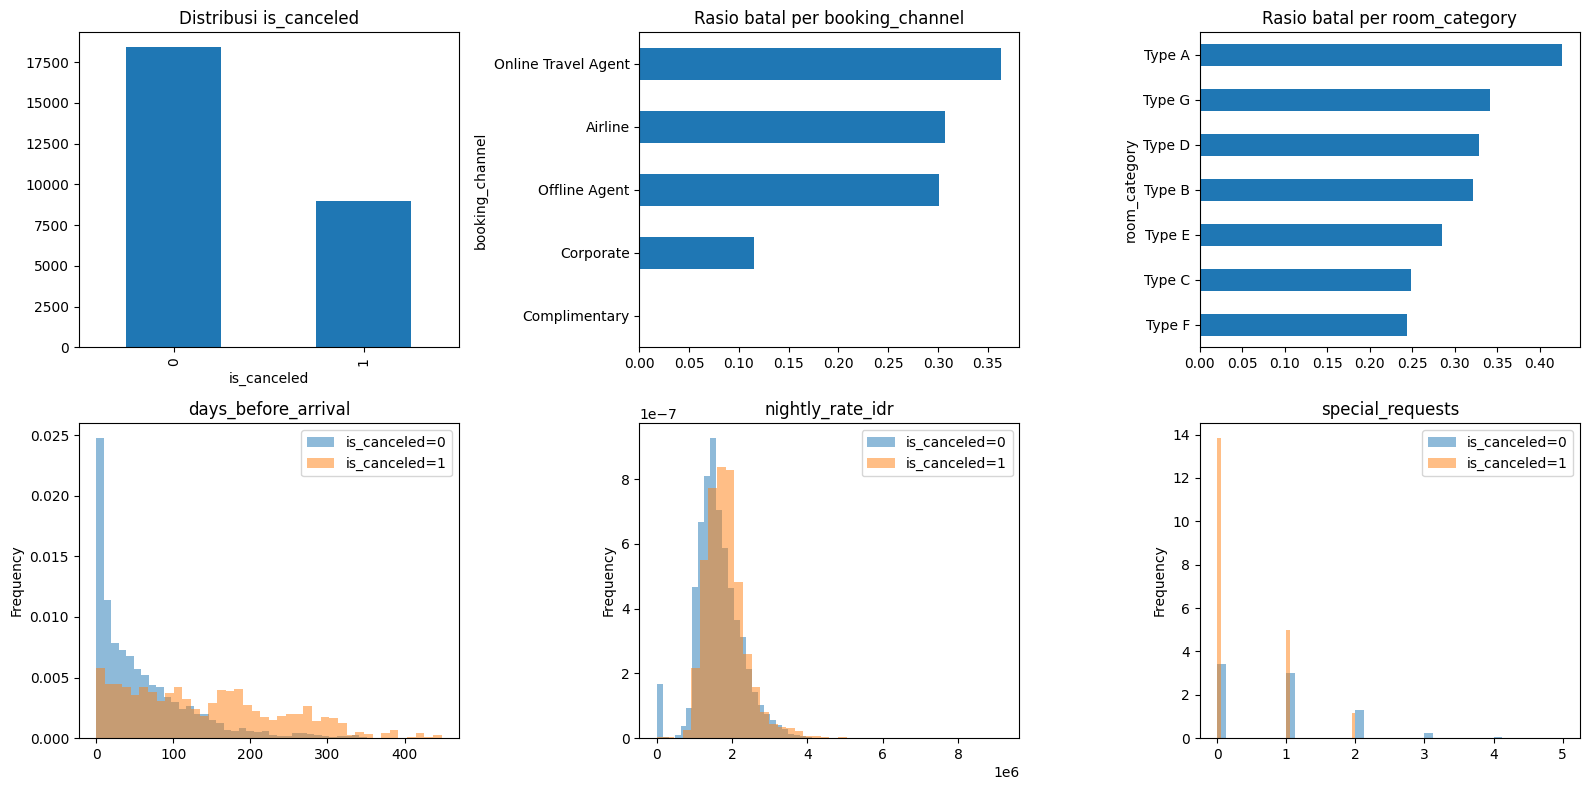
\includegraphics[width=0.95\textwidth]{assets/eda_overview.png}
  \caption{Eksplorasi awal dataset pemesanan penginapan: distribusi kelas target, korelasi \texttt{days\_before\_arrival} terhadap pembatalan, pengaruh \texttt{special\_requests}, kanal pemesanan, dan distribusi tarif malam.}
  \label{fig:eda}
\end{figure}

Berdasarkan eksplorasi awal pada Gambar~\ref{fig:eda}, terdapat tiga karakteristik penting pada dataset:
\begin{enumerate}[leftmargin=1.4cm, itemsep=2pt]
  \item \textbf{Ketidakseimbangan kelas moderat}: rasio pemesanan tidak batal mencapai \textbf{67,23\%} (18.404 baris), sedangkan pemesanan batal sebesar \textbf{32,77\%} (8.969 baris). Oleh karena itu, metrik evaluasi utama yang digunakan adalah \textbf{Macro F1-Score} agar kinerja pada kelas minoritas dan mayoritas dinilai secara seimbang\fnmark{1}.
  \item \textbf{Nilai kosong bersifat informatif (MNAR)}: terdapat 8 kolom dengan nilai kosong (\textit{missing values}), tertinggi pada \texttt{num\_children} (11,09\%), \texttt{special\_requests} (9,13\%), dan \texttt{nightly\_rate\_idr} (7,45\%). Rasio pembatalan ketika \texttt{special\_requests} kosong mencapai \textbf{40,7\%}, jauh lebih tinggi dibanding ketika terisi (32,0\%).
  \item \textbf{Pola prediktif kuat}: fitur yang paling berkorelasi dengan pembatalan adalah \texttt{days\_before\_arrival} ($r = 0{,}440$). Pemesanan dengan jarak waktu panjang ($>180$ hari) memiliki rasio batal 72,2\%, sementara pemesanan dengan \texttt{special\_requests} $\ge 3$ hampir tidak pernah dibatalkan (0,0\%).
\end{enumerate}

Tujuan utama dari pengerjaan Tugas Besar 2 ini adalah:
\begin{enumerate}[leftmargin=1.4cm, itemsep=2pt]
  \item Merancang alur pengolahan data (\textit{cleaning}, transformasi, \textit{feature selection}, dan evaluasi reduksi dimensi) secara terpisah antara data latih dan data uji tanpa kebocoran data (\textit{data leakage}).
  \item Mengimplementasikan lima algoritma \textit{supervised learning} dari awal (\textit{from scratch}) hanya menggunakan pustaka matematika (\texttt{NumPy}) dan pustaka standar Python: \textbf{KNN}, \textbf{Decision Tree Learning (CART)}, \textbf{Logistic Regression} (L1, L2, Elastic Net), \textbf{SVM} (Linear, Polynomial, Gaussian), dan \textbf{Bayesian Network / Naive Bayes}\fnmark{3}.
  \item Membandingkan kinerja kelima algoritma \textit{from scratch} terhadap implementasi \texttt{scikit-learn}, memverifikasi mekanisme \textit{save/load} model, melakukan analisis \textit{cost-sensitive} ($C_{\text{FP}} = 2 \cdot C_{\text{FN}}$), serta menghasilkan submisi Kaggle tunggal (\textit{non-ensemble}) yang \textit{reproducible}.
\end{enumerate}

\begin{footnoteinfo}
  \item \textbf{Tim Asisten IF3170}, ``\textit{Spesifikasi Tugas Besar 2: Supervised Learning IF3170 Inteligensi Artifisial}'', Program Studi Teknik Informatika, Institut Teknologi Bandung, 2026.
  \item \textbf{S. Russell dan P. Norvig}, ``\textit{Artificial Intelligence: A Modern Approach}'', edisi ke-4, Pearson, 2020.
  \item \textbf{Tim Pengajar IF3170}, ``\textit{Supervised Learning (KNN, DTL, Logistic Regression, SVM, Naive Bayes): Bahan Kuliah IF3170 Inteligensi Artifisial}'', Program Studi Teknik Informatika, Sekolah Teknik Elektro dan Informatika, Institut Teknologi Bandung, 2026.
\end{footnoteinfo}

% =====================================================================
% BAB 2: PEMBAHASAN DAN ANALISA
% =====================================================================
\clearpage
\section{Pembahasan dan Analisa}

Pada bagian ini dibahas rancangan pengolahan data, implementasi kelima algoritma \textit{supervised learning} beserta potongan kode sumbernya, perbandingan eksperimen dengan pustaka \texttt{scikit-learn}, analisis \textit{cost-sensitive}, serta \textit{error analysis}.

% ---------------------------------------------------------------------
\subsection[Tahapan Pengolahan Data]{Tahapan Pengolahan Data (\texttt{src/preprocessing.py})}

Seluruh alur prapemrosesan data dikemas dalam kelas \texttt{DataPreprocessor} pada \texttt{src/preprocessing.py}. Prinsip utama yang ditegakkan di seluruh eksperimen adalah \textbf{pemisahan ketat antara data latih dan data uji}: seluruh statistik (median, modus, rata-rata, simpangan baku, daftar kategori, dan bobot seleksi fitur) dihitung secara eksklusif melalui \texttt{fit()} pada data latih (\texttt{train\_set} 80\% terstratifikasi, atau setiap \textit{training fold} pada \textit{5-fold Stratified CV}), lalu diterapkan ke data validasi dan data uji melalui \texttt{transform()}.

\subsubsection{Data Cleaning}
\begin{itemize}[leftmargin=1.2cm, itemsep=2pt]
  \item \textbf{Penanganan Nilai Kosong}: Karena pola kekosongan berkorelasi dengan target (contoh: \texttt{special\_requests} kosong memiliki rasio batal 40,7\%), ditambahkan 8 kolom indikator biner \texttt{<kolom>\_is\_missing}. Untuk model berbasis jarak/linear/SVM, nilai kosong numerik diimputasi menggunakan median data latih dan kategorikal menggunakan modus data latih. Khusus jalur \textbf{DTL} (\texttt{mode='dtl\_ready'}), nilai \texttt{NaN} dipertahankan apa adanya agar ditangani secara internal oleh algoritma pohon keputusan.
  \item \textbf{Penanganan Duplikat}: Ditemukan 64 baris duplikat pada data latih penuh (40 baris pada \texttt{train\_set} 80\%, termasuk 2 baris dengan fitur identik tetapi label berlawanan). Penghapusan duplikat (\texttt{clean\_training\_dataframe}) hanya diterapkan pada data latih sehingga ukuran \texttt{train\_set} berubah dari 21.898 menjadi 21.858 baris, sedangkan \texttt{val\_set} (5.475 baris) dan \texttt{test.csv} (6.844 baris) tidak pernah dihapus barisnya.
  \item \textbf{Penanganan Outlier dan Data Error}: Pemeriksaan IQR menandai banyak nilai ekstrem yang sah secara bisnis (misalnya lama menginap panjang dan riwayat pembatalan tinggi), sehingga tidak dilakukan pemangkasan buta. Sebaliknya, nilai yang mustahil secara domain (pemesanan dengan total tamu = 0 dan \texttt{nightly\_rate\_idr} negatif) diubah menjadi \texttt{NaN} lalu diimputasi.
\end{itemize}

\subsubsection{Data Transformation, Feature Selection, dan Dimensionality Reduction}
\begin{itemize}[leftmargin=1.2cm, itemsep=2pt]
  \item \textbf{Konstruksi Fitur Domain}: Dari 17 fitur awal dibentuk fitur turunan yang bermakna secara bisnis, antara lain \texttt{total\_guests}, \texttt{total\_nights}, \texttt{weekend\_ratio}, \texttt{total\_booking\_cost}, \texttt{has\_prior\_history}, \texttt{prior\_cancel\_rate}, \texttt{arrival\_dayofweek}, serta transformasi logaritmik pada fitur miring (\textit{skewed}). Untuk Logistic Regression teroptimasi, ditambahkan interaksi komposit dan transformasi non-linear (982 fitur), sedangkan untuk Naive Bayes TAN + CLL digunakan fitur diskrit multi-resolusi.
  \item \textbf{Encoding dan Scaling}: Fitur kategorikal (\texttt{meal\_package}, \texttt{room\_category}, \texttt{booking\_channel}) di-\textit{encode} menggunakan \textit{One-Hot Encoding} untuk KNN, Logistic Regression, dan SVM agar tidak menimbulkan urutan artifisial. Fitur numerik distandardisasi ($z = (x-\mu)/\sigma$) menggunakan parameter dari data latih.
  \item \textbf{Penanganan Ketidakseimbangan Kelas}: Diuji tiga metode \textit{resampling} pada \texttt{train\_set} menggunakan baseline Logistic Regression (Tabel~\ref{tab:resampling}). Seluruh metode \textit{resampling} menaikkan \textit{recall} kelas batal (dari 0,6148 menjadi $\sim$0,764), tetapi menurunkan \textit{precision} (0,7324 $\rightarrow$ 0,630) sehingga \textbf{Macro F1 justru menurun} (0,7627 $\rightarrow$ 0,7565--0,7579). Oleh karena itu, model final dilatih tanpa \textit{resampling} dan ketidakseimbangan ditangani melalui \textit{threshold tuning} pada probabilitas OOF.
  \item \textbf{Feature Selection dan PCA}: Seleksi fitur berbasis mRMR (\textit{minimum Redundancy Maximum Relevance}) diimplementasikan pada \texttt{\_select\_mrmr\_features}. Selain itu, reduksi dimensi \textbf{PCA} diuji pada 95\% varians (30 komponen) dan 80\% varians (21 komponen) seperti pada Tabel~\ref{tab:pca}. Karena PCA menurunkan Macro F1 (dari 0,7627 menjadi 0,7597 dan 0,7302) sekaligus menghilangkan interpretabilitas fitur, PCA tidak dipakai pada pipeline model utama dan hanya dimanfaatkan untuk visualisasi 2D SVM.
\end{itemize}

\begin{table}[H]
  \centering
  \small
  \setlength{\tabcolsep}{4pt}
  \caption{Perbandingan metode penanganan ketidakseimbangan kelas pada \texttt{val\_set} (baseline Logistic Regression).}
  \label{tab:resampling}
  \begin{tabularx}{\textwidth}{|Y|R{1.6cm}|R{1.8cm}|R{1.6cm}|R{1.7cm}|R{1.5cm}|R{1.7cm}|}
    \hline
    \rowcolor{tblblue}
    \textbf{Metode Resampling} & \textbf{N Latih} & \textbf{Rasio Pos.} & \textbf{Accuracy} & \textbf{Precision} & \textbf{Recall} & \textbf{Macro F1} \\
    \hline
    Tanpa resampling (\texttt{none}) & 21.858 & 0,3277 & \textbf{0,8002} & \textbf{0,7324} & 0,6148 & \textbf{0,7627} \\
    \hline
    Random Oversampling & 29.392 & 0,5000 & 0,7763 & 0,6308 & 0,7648 & 0,7579 \\
    \hline
    Random Undersampling & 14.324 & 0,5000 & 0,7750 & 0,6289 & 0,7642 & 0,7567 \\
    \hline
    SMOTE & 29.392 & 0,5000 & 0,7750 & 0,6294 & 0,7620 & 0,7565 \\
    \hline
  \end{tabularx}
\end{table}

\begin{table}[H]
  \centering
  \small
  \setlength{\tabcolsep}{6pt}
  \caption{Pengaruh reduksi dimensi PCA terhadap performa Logistic Regression baseline pada \texttt{val\_set}.}
  \label{tab:pca}
  \begin{tabularx}{\textwidth}{|Y|R{2.4cm}|R{2.2cm}|R{2.2cm}|R{2.2cm}|}
    \hline
    \rowcolor{tblblue}
    \textbf{Konfigurasi} & \textbf{Jumlah Fitur} & \textbf{Accuracy} & \textbf{Macro F1} & \textbf{ROC-AUC} \\
    \hline
    Tanpa PCA & 59 & \textbf{0,8002} & \textbf{0,7627} & \textbf{0,8597} \\
    \hline
    PCA 95\% varians & 30 & 0,7995 & 0,7597 & 0,8566 \\
    \hline
    PCA 80\% varians & 21 & 0,7823 & 0,7302 & 0,8319 \\
    \hline
  \end{tabularx}
\end{table}

% ---------------------------------------------------------------------
\subsection{Implementasi Algoritma \textit{From Scratch} dan Utilitas}

Kelima algoritma diimplementasikan murni menggunakan \texttt{NumPy} dan pustaka standar Python (tanpa \texttt{scikit-learn} maupun \texttt{scipy} di dalam kelas model) serta mendukung serialisasi \texttt{save()}/\texttt{load()}.

\subsubsection[K-Nearest Neighbors]{K-Nearest Neighbors (\texttt{src/models/knn.py})}

Kelas \texttt{KNN} mengimplementasikan \textit{lazy learning} dengan dukungan metrik jarak \textit{Euclidean} ($L_2$), \textit{Manhattan} ($L_1$), dan \textit{Minkowski} ($L_p$), pembobotan tetangga \texttt{uniform} maupun \texttt{distance} ($w_i = 1/(d_i + \varepsilon)$), serta \textbf{pembobotan fitur} (\textit{feature weighting})\fnmark{4} dan optimasi \textit{threshold} probabilitas\fnmark{5}. Perhitungan jarak dilakukan secara \textit{batched} (\texttt{batch\_size=256}) agar hemat memori. Konfigurasi terbaik menggunakan $k=25$, jarak \textit{Manhattan}, \texttt{weights='distance'}, dan \textit{threshold} $0{,}48$.

\noindent\begin{minipage}{\linewidth}
\begin{lstlisting}
class KNN:
    def __init__(self, n_neighbors=5, metric="euclidean", p=2,
                 weights="uniform", feature_weights=None, batch_size=256):
        self.n_neighbors = int(n_neighbors)
        self.metric = metric
        self.p = float(p)
        self.weights = weights
        self.feature_weights = feature_weights
        self.batch_size = int(batch_size)

    def _compute_distances(self, X_batch):
        if self.metric == "manhattan":
            return np.sum(np.abs(X_batch[:, None, :] - self.X_train_[None, :, :]), axis=2)
        if self.metric == "euclidean":
            sq = (np.sum(X_batch ** 2, axis=1, keepdims=True)
                  + np.sum(self.X_train_ ** 2, axis=1)
                  - 2.0 * (X_batch @ self.X_train_.T))
            return np.sqrt(np.maximum(sq, 0.0))
        return np.sum(np.abs(X_batch[:, None, :] - self.X_train_[None, :, :]) ** self.p,
                      axis=2) ** (1.0 / self.p)
\end{lstlisting}
\end{minipage}

\subsubsection[Decision Tree Learning -- CART/Entropy]{Decision Tree Learning -- CART/Entropy (\texttt{src/models/dtl.py})}

Kelas \texttt{DecisionTree} mengimplementasikan varian CART dengan pilihan kriteria impuritas \texttt{gini} dan \texttt{entropy}\fnmark{6}. Empat kemampuan utama yang dibangun secara native:
\begin{enumerate}[leftmargin=1.4cm, itemsep=2pt]
  \item \textbf{Fitur Numerik}: pemisahan biner $x \le t$ dengan kandidat kuantil tervektorisasi (\texttt{n\_bins=64}).
  \item \textbf{Fitur Kategorikal}: \textit{optimal binary subset split} $x \in S$ dengan mengurutkan kategori berdasarkan proporsi kelas positif $P(y=1 \mid x=c)$\fnmark{6} sehingga kompleksitas berkurang dari $O(2^{M-1})$ menjadi $O(M \log M)$.
  \item \textbf{Penanganan Nilai Kosong (\texttt{NaN}) Internal}: tanpa imputasi luar, mendukung mode \texttt{learned} (\textit{sparsity-aware default direction})\fnmark{8} yang mempelajari arah cabang optimal (kiri/kanan) untuk \texttt{NaN} pada tiap simpul, serta mode \texttt{c45} (pembobotan proporsional)\fnmark{7}.
  \item \textbf{Bonus Optimasi \& Visualisasi}: \textit{Minimal Cost-Complexity Pruning} (\texttt{ccp\_alpha}, \textit{weakest-link pruning}) berbasis \textit{bottom-up dynamic programming} $O(N)$, serta metode \texttt{plot\_tree(top\_n=3)} untuk memvisualisasikan percabangan teratas pohon.
\end{enumerate}

\noindent\begin{minipage}{\linewidth}
\begin{lstlisting}
def _prune(self, root: dict, alpha: float) -> dict:
    # Sumber: Breiman et al. (1984) Ch. 3.3 - Minimal Cost-Complexity Pruning
    if alpha <= 0.0 or not root:
        return root
    root = copy.deepcopy(root)
    while not root["leaf"]:
        best = [np.inf, None]
        def walk(nd: dict) -> Tuple[int, float]:
            if nd["leaf"]:
                return 1, nd["risk"]
            ll, lr = walk(nd["left"])
            rl, rr = walk(nd["right"])
            leaves, sub_risk = ll + rl, lr + rr
            g = (nd["risk"] - sub_risk) / max(leaves - 1, 1)
            if g < best[0]:
                best[0], best[1] = g, nd
            return leaves, sub_risk
        walk(root)
        if best[1] is None or best[0] > alpha:
            break
        for k in ("f", "t", "cat", "cats", "left", "right", "ndir"):
            best[1].pop(k, None)
        best[1]["leaf"] = True
    return root
\end{lstlisting}
\end{minipage}

\subsubsection[Logistic Regression]{Logistic Regression (\texttt{src/models/logistic\_regression.py})}

Kelas \texttt{LogisticRegression} memaksimalkan \textit{regularized log-likelihood} dengan dukungan penuh tiga skema regularisasi wajib: \textbf{L1} (Lasso), \textbf{L2} (Ridge), dan \textbf{Elastic Net}\fnmark{9} beserta mode tanpa penalti (\texttt{none}). Untuk optimasi (bonus), diimplementasikan tiga algoritma: \textit{Stochastic Gradient Ascent} (SGA), \textbf{Adam}\fnmark{10} dengan \textit{proximal soft-thresholding} untuk penalti L1, dan \textbf{L-BFGS}\fnmark{11} berbasis \textit{two-loop recursion} dengan \textit{backtracking Armijo line search}. Selain itu, metode \texttt{animate\_loss\_contour()} menghasilkan animasi GIF lintasan parameter $(\theta_0, \theta_1)$ pada permukaan kontur \textit{log-loss}.

\noindent\begin{minipage}{\linewidth}
\begin{lstlisting}
def _l1_l2_strength(self) -> Tuple[float, float]:
    if self.penalty == "none":
        return 0.0, 0.0
    if self.penalty == "l1":
        return self.reg_lambda, 0.0
    if self.penalty == "l2":
        return 0.0, self.reg_lambda
    return self.reg_lambda * self.l1_ratio, self.reg_lambda * (1.0 - self.l1_ratio)

def _fit_lbfgs(self, X: np.ndarray, y: np.ndarray) -> None:
    # Two-loop recursion L-BFGS (Nocedal & Wright, 2006) + Armijo line search
    m = self.lbfgs_history
    s_hist, y_hist, rho_hist = [], [], []
    for _ in range(self.max_iter):
        grad_ll = self._likelihood_gradient(X, y)
        g = -grad_ll
        if np.max(np.abs(g)) < self.tol:
            break
        q = g.copy()
        alphas = []
        for s, yk, rho in zip(reversed(s_hist), reversed(y_hist), reversed(rho_hist)):
            a = rho * float(np.dot(s, q))
            alphas.append(a); q -= a * yk
        gamma = (float(np.dot(s_hist[-1], y_hist[-1])) /
                 max(float(np.dot(y_hist[-1], y_hist[-1])), 1e-12)) if s_hist else 1.0
        r = gamma * q
        for s, yk, rho, a in zip(s_hist, y_hist, rho_hist, reversed(alphas)):
            r += s * (a - rho * float(np.dot(yk, r)))
        step_dir = -r
\end{lstlisting}
\end{minipage}

\subsubsection[Support Vector Machine]{Support Vector Machine (\texttt{src/models/svm.py})}

Kelas \texttt{SVM} menyelesaikan formulasi dual \textit{soft-margin SVM} menggunakan algoritma \textbf{Sequential Minimal Optimization (SMO)}\fnmark{12} yang dipercepat dengan \textbf{Working Set Selection orde-dua (WSS2)}\fnmark{13}, mekanisme \textbf{\textit{shrinking}} variabel aktif, serta \textit{LRU kernel row cache}. Tiga fungsi kernel wajib diimplementasikan dalam kelas \texttt{Kernel}:
\begin{itemize}[leftmargin=1.2cm, itemsep=1pt]
  \item \textbf{Linear}: $K(x, z) = x^\top z$
  \item \textbf{Polynomial}: $K(x, z) = (\gamma x^\top z + r)^d$
  \item \textbf{Gaussian (RBF)}: $K(x, z) = \exp(-\gamma \|x - z\|_2^2)$
\end{itemize}

\noindent\begin{minipage}{\linewidth}
\begin{lstlisting}
class Kernel:
    def __init__(self, kind: str = "rbf", gamma: float = 1.0,
                 degree: int = 3, coef0: float = 0.0):
        self.kind = kind
        self.gamma = float(gamma)
        self.degree = int(degree)
        self.coef0 = float(coef0)

    def __call__(self, X: np.ndarray, Z: np.ndarray) -> np.ndarray:
        if self.kind == "linear":
            return X @ Z.T
        if self.kind == "poly":
            return (self.gamma * (X @ Z.T) + self.coef0) ** self.degree
        x2 = np.sum(X * X, axis=1, keepdims=True)
        z2 = np.sum(Z * Z, axis=1)[None, :]
        return np.exp(-self.gamma * np.maximum(x2 + z2 - 2.0 * (X @ Z.T), 0.0))
\end{lstlisting}
\end{minipage}

\subsubsection[Bayesian Network / Naive Bayes]{Bayesian Network / Naive Bayes (\texttt{src/models/naive\_bayes.py})}

Kelas \texttt{NaiveBayes} mendukung tiga mode probabilistik secara terpadu: (1) \textbf{Gaussian Naive Bayes} untuk fitur kontinu, (2) \textbf{Categorical Naive Bayes} dengan \textit{Laplace/Dirichlet smoothing} sesuai salindia kuliah\fnmark{3}, dan (3) \textbf{Bayesian Network teroptimasi (TAN + CLL)} yang mengombinasikan \textit{Tree-Augmented Naive Bayes} berbasis pohon rentang maksimum \textbf{Chow-Liu}\fnmark{14}\fnmark{15} menggunakan \textit{Conditional Mutual Information (CMI)}, dependensi $k$-DB/HNB/SP2DE\fnmark{16}\fnmark{17}\fnmark{18}, estimasi densitas kernel Parzen, serta kalibrasi bobot \textit{Conditional Log-Likelihood (CLL)} via L-BFGS. Visualisasi struktur graf berarah dihasilkan melalui \texttt{plot\_network\_graph()} menggunakan \texttt{src/utils/network\_plot.py}.

\noindent\begin{minipage}{\linewidth}
\begin{lstlisting}
def _build_chow_liu_mwst(self, cmi_matrix: np.ndarray, root_idx: int) -> np.ndarray:
    # Algoritma Prim untuk Maximum Weight Spanning Tree (Chow & Liu, 1968)
    n_features = cmi_matrix.shape[0]
    parents = np.full(n_features, -1, dtype=int)
    in_tree = np.zeros(n_features, dtype=bool)
    in_tree[root_idx] = True
    for _ in range(n_features - 1):
        best_w, best_u, best_v = -1.0, -1, -1
        for u in np.flatnonzero(in_tree):
            for v in np.flatnonzero(~in_tree):
                if cmi_matrix[u, v] > best_w:
                    best_w, best_u, best_v = cmi_matrix[u, v], u, v
        if best_v == -1:
            break
        in_tree[best_v] = True
        parents[best_v] = best_u
    return parents
\end{lstlisting}
\end{minipage}

\subsubsection[Utilitas Serialisasi dan Evaluasi]{Utilitas Serialisasi dan Evaluasi (\texttt{model\_io.py} \& \texttt{metrics.py})}

Modul \texttt{src/utils/model\_io.py} menyediakan fungsi standar \texttt{save\_model()} dan \texttt{load\_model()} berbasis \texttt{pickle} untuk menyimpan dan memuat kembali seluruh model ke \texttt{output/models/}. Sementara itu, \texttt{src/utils/metrics.py} mengimplementasikan seluruh metrik klasifikasi (\texttt{accuracy}, \texttt{precision}, \texttt{recall}, \texttt{f1\_macro}, \texttt{roc\_auc}, \texttt{confusion\_matrix}), fungsi \texttt{prediction\_agreement()}, serta rangkaian evaluasi \textit{cost-sensitive} secara murni dengan \texttt{NumPy}.

% ---------------------------------------------------------------------
\subsection{Hasil Eksperimen, Perbandingan dengan \texttt{scikit-learn}, dan Visualisasi}

\subsubsection{Ringkasan Performa 5 Model \textit{From Scratch}}

Seluruh lima model \textit{from scratch} dievaluasi pada himpunan validasi \texttt{val\_set} 20\% (5.475 baris) yang identik agar perbandingannya setara (\textit{apples-to-apples}), lalu dilatih ulang pada seluruh data latih bersih (27.309 baris) untuk menghasilkan submisi pada Kaggle Public Leaderboard (6.844 baris uji). Ringkasan hasil disajikan pada Tabel~\ref{tab:summary5} dan Gambar~\ref{fig:summary5}.

\begin{table}[H]
  \centering
  \small
  \setlength{\tabcolsep}{4pt}
  \caption{Ringkasan performa 5 model \textit{from scratch} pada \texttt{val\_set} 20\% dan Kaggle Public Leaderboard.}
  \label{tab:summary5}
  \begin{tabularx}{\textwidth}{|Y|R{1.3cm}|R{1.3cm}|R{1.3cm}|R{1.4cm}|R{1.3cm}|R{1.65cm}|}
    \hline
    \rowcolor{tblblue}
    \textbf{Model (\textit{From Scratch})} & \textbf{Acc.} & \textbf{Prec.} & \textbf{Rec.} & \textbf{Val F1} & \textbf{AUC} & \textbf{Kaggle LB} \\
    \hline
    \textbf{NB TAN + CLL (Utama)} & \textbf{0,8895} & \textbf{0,8614} & \textbf{0,7899} & \textbf{0,8718} & \textbf{0,9508} & \textbf{0,87066} \\
    \hline
    Logistic Regression (L-BFGS Opt) & 0,8796 & 0,8392 & 0,7826 & 0,8609 & 0,9405 & 0,86410 \\
    \hline
    KNN Berbobot Fitur ($k=25, L_1$) & 0,8703 & 0,8140 & 0,7832 & 0,8514 & 0,9350 & 0,85633 \\
    \hline
    SVM Gaussian ($C=10, t=-0{,}3$) & 0,8581 & 0,7811 & 0,7876 & 0,8393 & 0,9158 & 0,85254 \\
    \hline
    DTL CART (Entropy + Pruning) & 0,8597 & 0,8032 & 0,7575 & 0,8384 & 0,8979 & 0,84226 \\
    \hline
  \end{tabularx}
\end{table}

\begin{figure}[H]
  \centering
  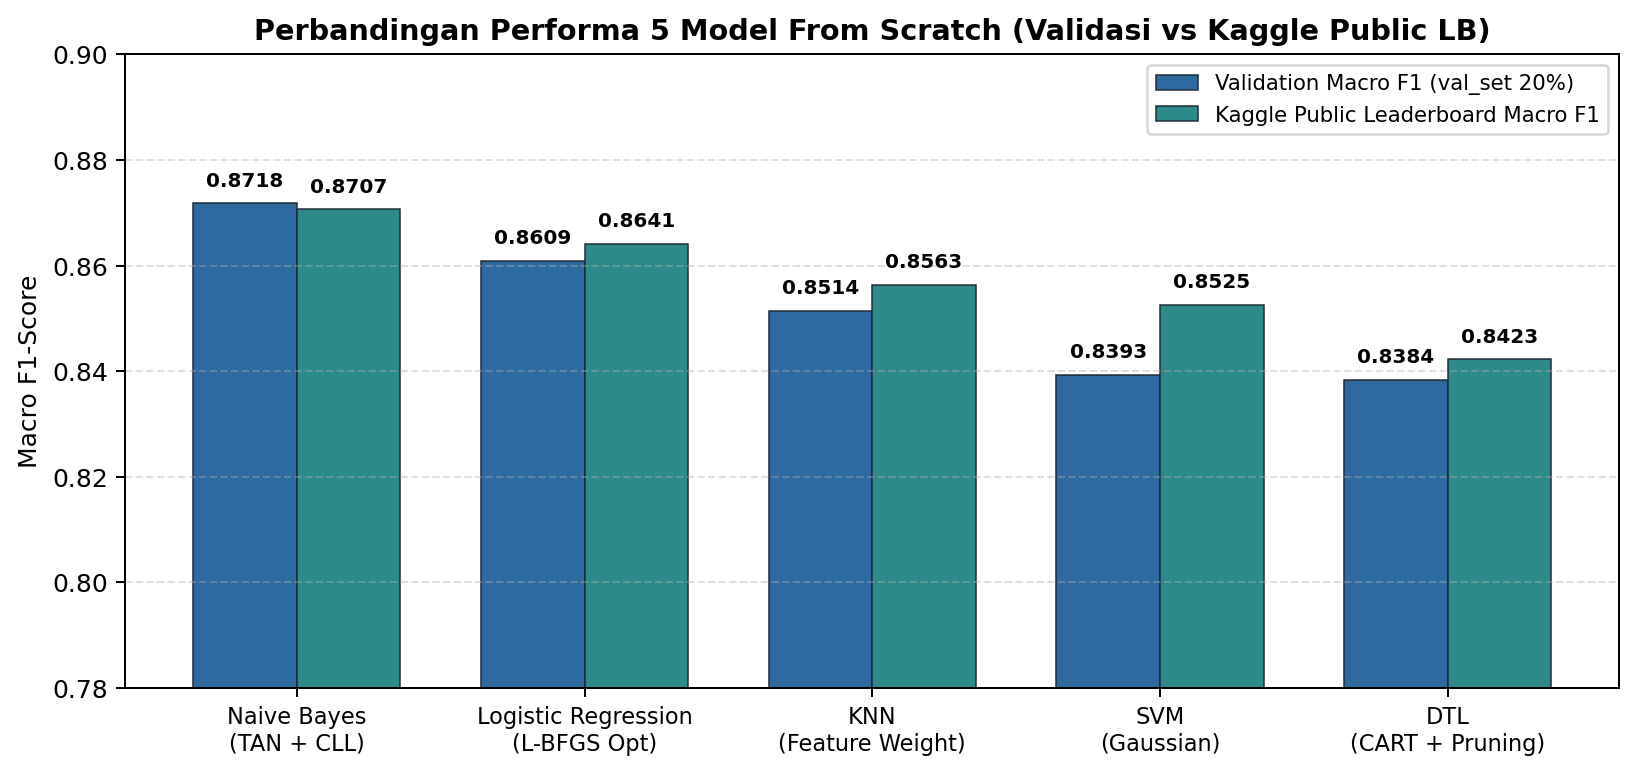
\includegraphics[width=0.90\textwidth]{assets/model_eval_comparison.png}
  \caption{Perbandingan Macro F1-Score lima model \textit{from scratch} pada \texttt{val\_set} 20\% dan Kaggle Public Leaderboard.}
  \label{fig:summary5}
\end{figure}

Peringkat kelima model pada validasi lokal konsisten 100\% dengan skor pada Kaggle Public Leaderboard, membuktikan tidak adanya kebocoran data maupun \textit{overfitting} parah. \textbf{Naive Bayes TAN + CLL} mencapai performa tertinggi dengan Macro F1 validasi \textbf{0,8718} dan Kaggle Public LB \textbf{0,87066} menggunakan satu model tunggal (\textit{non-ensemble}).

\subsubsection{Hasil dan Perbandingan KNN vs \texttt{scikit-learn}}

Pada Tabel~\ref{tab:knn}, penerapan pembobotan fitur meningkatkan Macro F1 KNN secara drastis sebesar $+0{,}0457$ (dari 0,8057 menjadi 0,8514) dan ROC-AUC dari 0,9028 menjadi 0,9350, karena fitur kurang relevan diberi bobot rendah/nol sehingga ruang jarak \textit{Manhattan} didominasi fitur paling diskriminatif. Perbandingan dengan \texttt{sklearn.neighbors.KNeighborsClassifier}\fnmark{20} menunjukkan \textbf{kesamaan prediksi 100,0000\%} dengan selisih probabilitas maksimum hanya $2{,}22 \times 10^{-16}$.

\begin{table}[H]
  \centering
  \small
  \setlength{\tabcolsep}{4pt}
  \caption{Evaluasi pembobotan fitur KNN dan perbandingan dengan \texttt{scikit-learn} pada \texttt{val\_set}.}
  \label{tab:knn}
  \begin{tabularx}{\textwidth}{|Y|L{2.55cm}|R{1.65cm}|R{1.65cm}|R{1.65cm}|R{1.65cm}|}
    \hline
    \rowcolor{tblblue}
    \textbf{Model} & \textbf{Implementasi} & \textbf{Accuracy} & \textbf{F1 Binary} & \textbf{Macro F1} & \textbf{ROC-AUC} \\
    \hline
    KNN tanpa bobot fitur & \texttt{from\_scratch} & 0,8385 & 0,7259 & 0,8057 & 0,9028 \\
    \hline
    KNN berbobot fitur & \texttt{from\_scratch} & \textbf{0,8703} & \textbf{0,7983} & \textbf{0,8514} & \textbf{0,9350} \\
    \hline
    KNN berbobot fitur & \texttt{scikit-learn} & 0,8703 & 0,7983 & 0,8514 & 0,9350 \\
    \hline
  \end{tabularx}
\end{table}

\subsubsection{Hasil dan Perbandingan DTL vs \texttt{scikit-learn} (ID3, C4.5, CART)}

Sesuai spesifikasi, DTL \textit{from scratch} dibandingkan terhadap tiga konfigurasi \texttt{DecisionTreeClassifier} pada \texttt{scikit-learn} (ID3 dengan \texttt{entropy}, C4.5 dengan \texttt{entropy + ccp\_alpha}, dan CART dengan \texttt{gini}) menggunakan protokol \textit{5-fold Stratified Cross-Validation} (Tabel~\ref{tab:dtl}). DTL \textit{from scratch} meraih \textbf{Macro F1 tertinggi (0,8316)} dan \textbf{Accuracy tertinggi (0,8552)}, mengungguli ketiga konfigurasi \texttt{scikit-learn}. Keunggulan ini berasal dari \textit{optimal binary subset split} untuk fitur kategorikal serta penanganan \texttt{NaN} secara internal (\texttt{learned}) yang tidak memaksa imputasi tunggal di luar pohon. Visualisasi percabangan teratas (\texttt{top\_n=3}) serta grafik perbandingan metrik, runtime, dan confusion matrix disajikan pada Gambar~\ref{fig:dtl_tree}, \ref{fig:dtl_metrics}, \ref{fig:dtl_rt}, dan~\ref{fig:dtl_cm}.

\begin{table}[H]
  \centering
  \small
  \setlength{\tabcolsep}{4pt}
  \caption{Perbandingan DTL \textit{from scratch} vs \texttt{scikit-learn} (ID3, C4.5, CART) pada 5-Fold Stratified CV.}
  \label{tab:dtl}
  \begin{tabularx}{\textwidth}{|Y|L{2.55cm}|R{1.25cm}|R{1.4cm}|R{1.35cm}|R{1.55cm}|R{1.25cm}|}
    \hline
    \rowcolor{tblblue}
    \textbf{Model} & \textbf{Implementasi} & \textbf{Acc.} & \textbf{Prec. M} & \textbf{Rec. M} & \textbf{Macro F1} & \textbf{Fit (s)} \\
    \hline
    \textbf{DTL Final (Entropy+CCP)} & \texttt{from\_scratch} & \textbf{0,8552} & \textbf{0,8413} & 0,8241 & \textbf{0,8316} & 32,96 \\
    \hline
    DTL ID3 (\texttt{entropy}) & \texttt{scikit-learn} & 0,8483 & 0,8305 & 0,8208 & 0,8252 & 0,46 \\
    \hline
    DTL C4.5 (\texttt{entropy+ccp}) & \texttt{scikit-learn} & 0,8510 & 0,8331 & \textbf{0,8252} & 0,8289 & 0,50 \\
    \hline
    DTL CART (\texttt{gini}) & \texttt{scikit-learn} & 0,8505 & 0,8322 & 0,8250 & 0,8284 & 0,43 \\
    \hline
  \end{tabularx}
\end{table}

\begin{figure}[H]
  \centering
  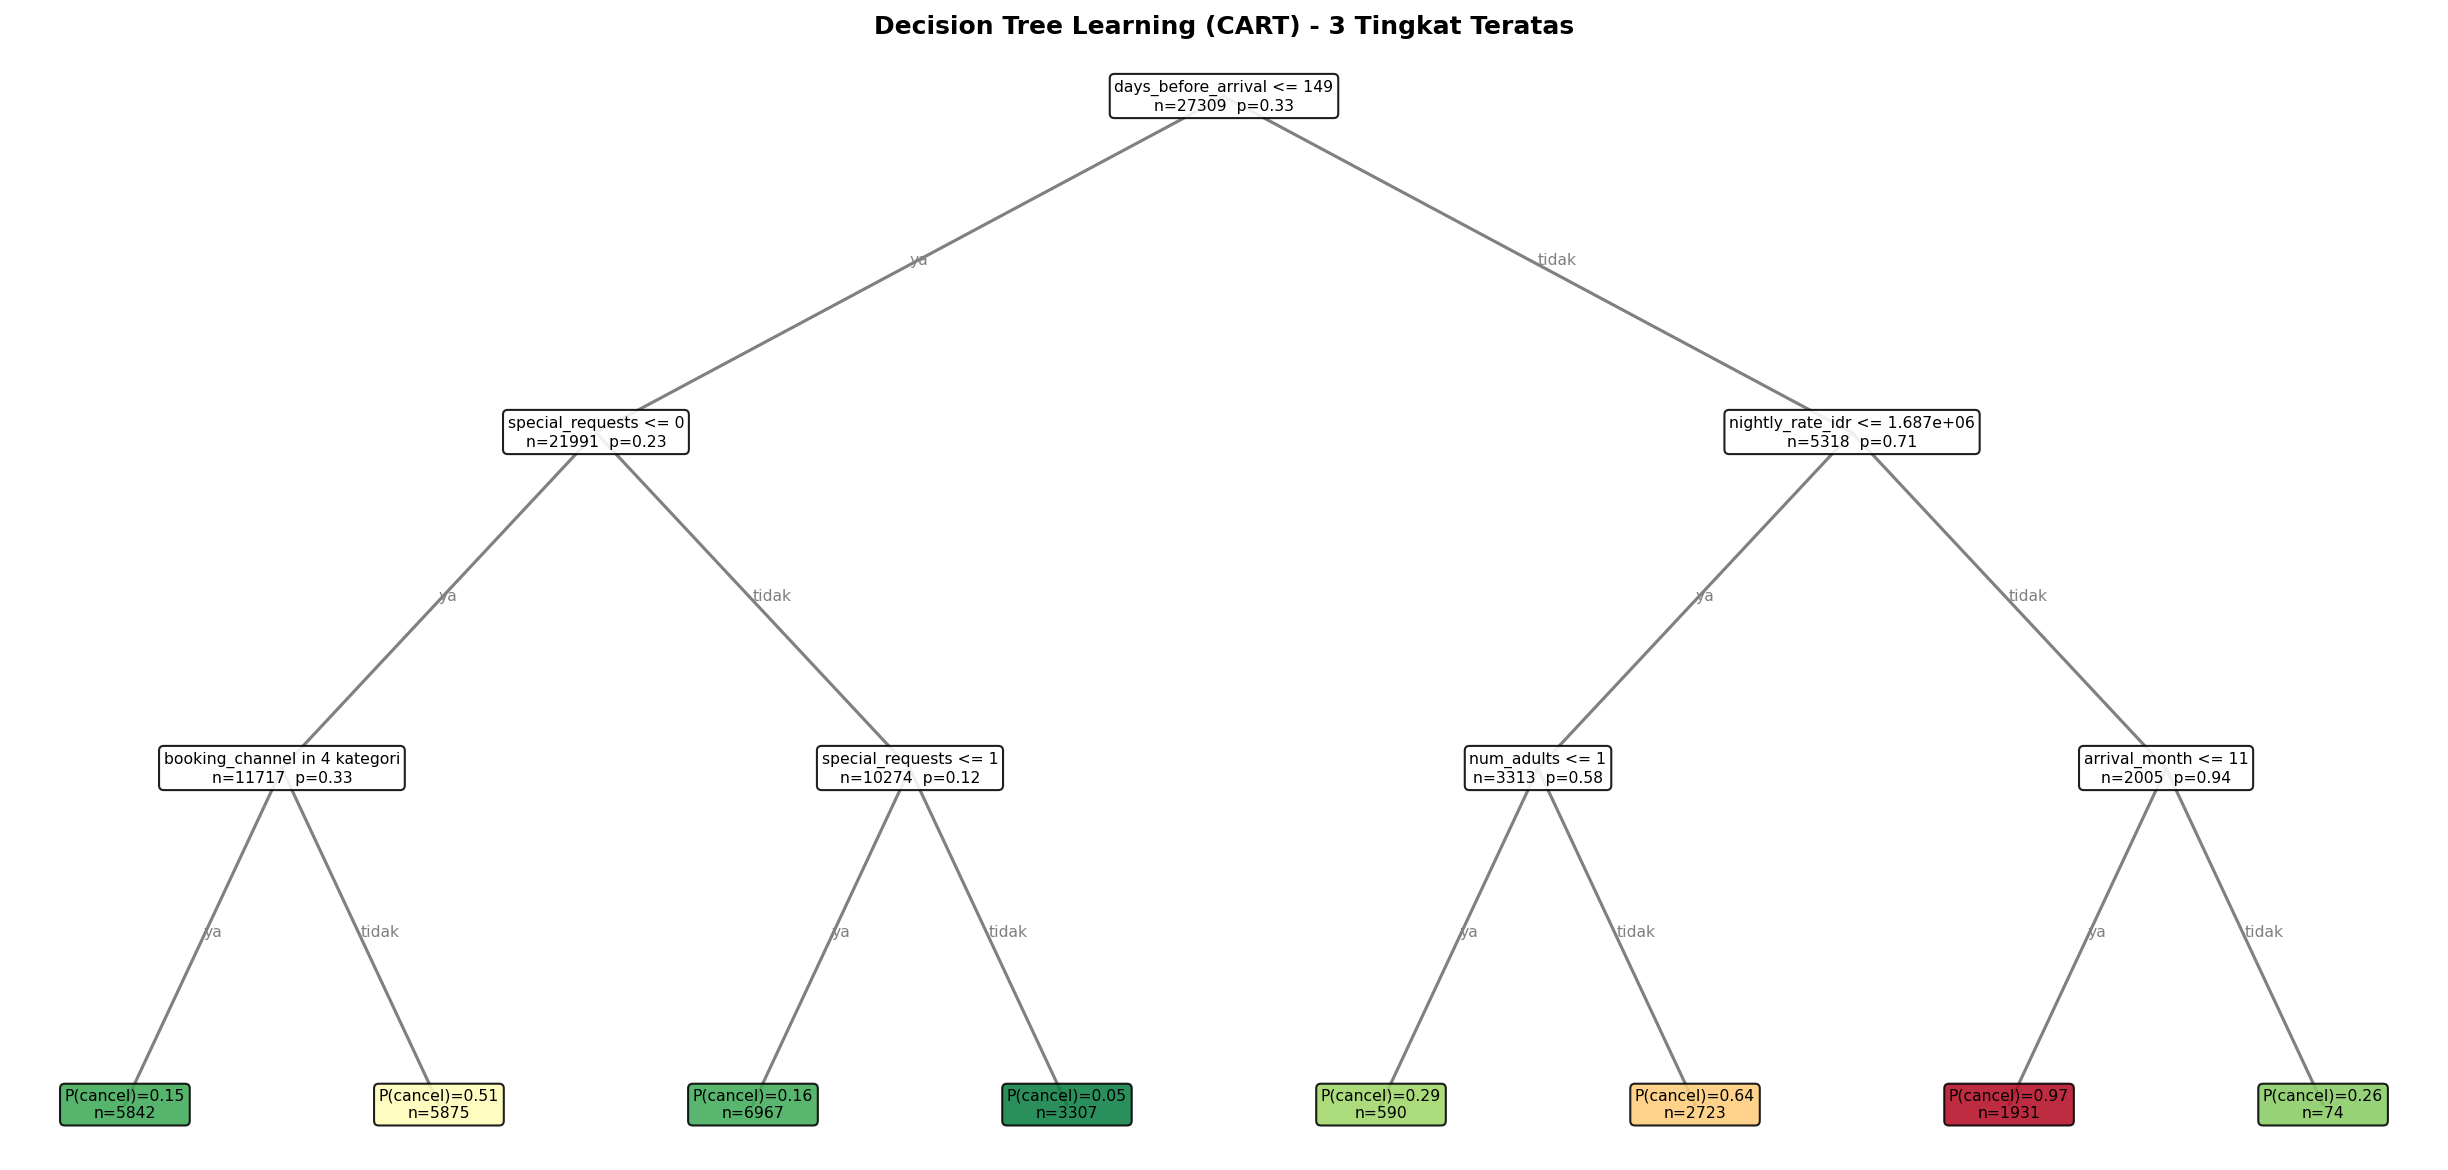
\includegraphics[width=0.92\textwidth]{assets/dtl_tree.png}
  \caption{Bonus visualisasi \texttt{top\_n=3} percabangan teratas pohon keputusan DTL \textit{from scratch} (\texttt{depth=21}, \texttt{leaves=250} setelah pruning \texttt{ccp\_alpha=0,0002}).}
  \label{fig:dtl_tree}
\end{figure}

\begin{figure}[H]
  \centering
  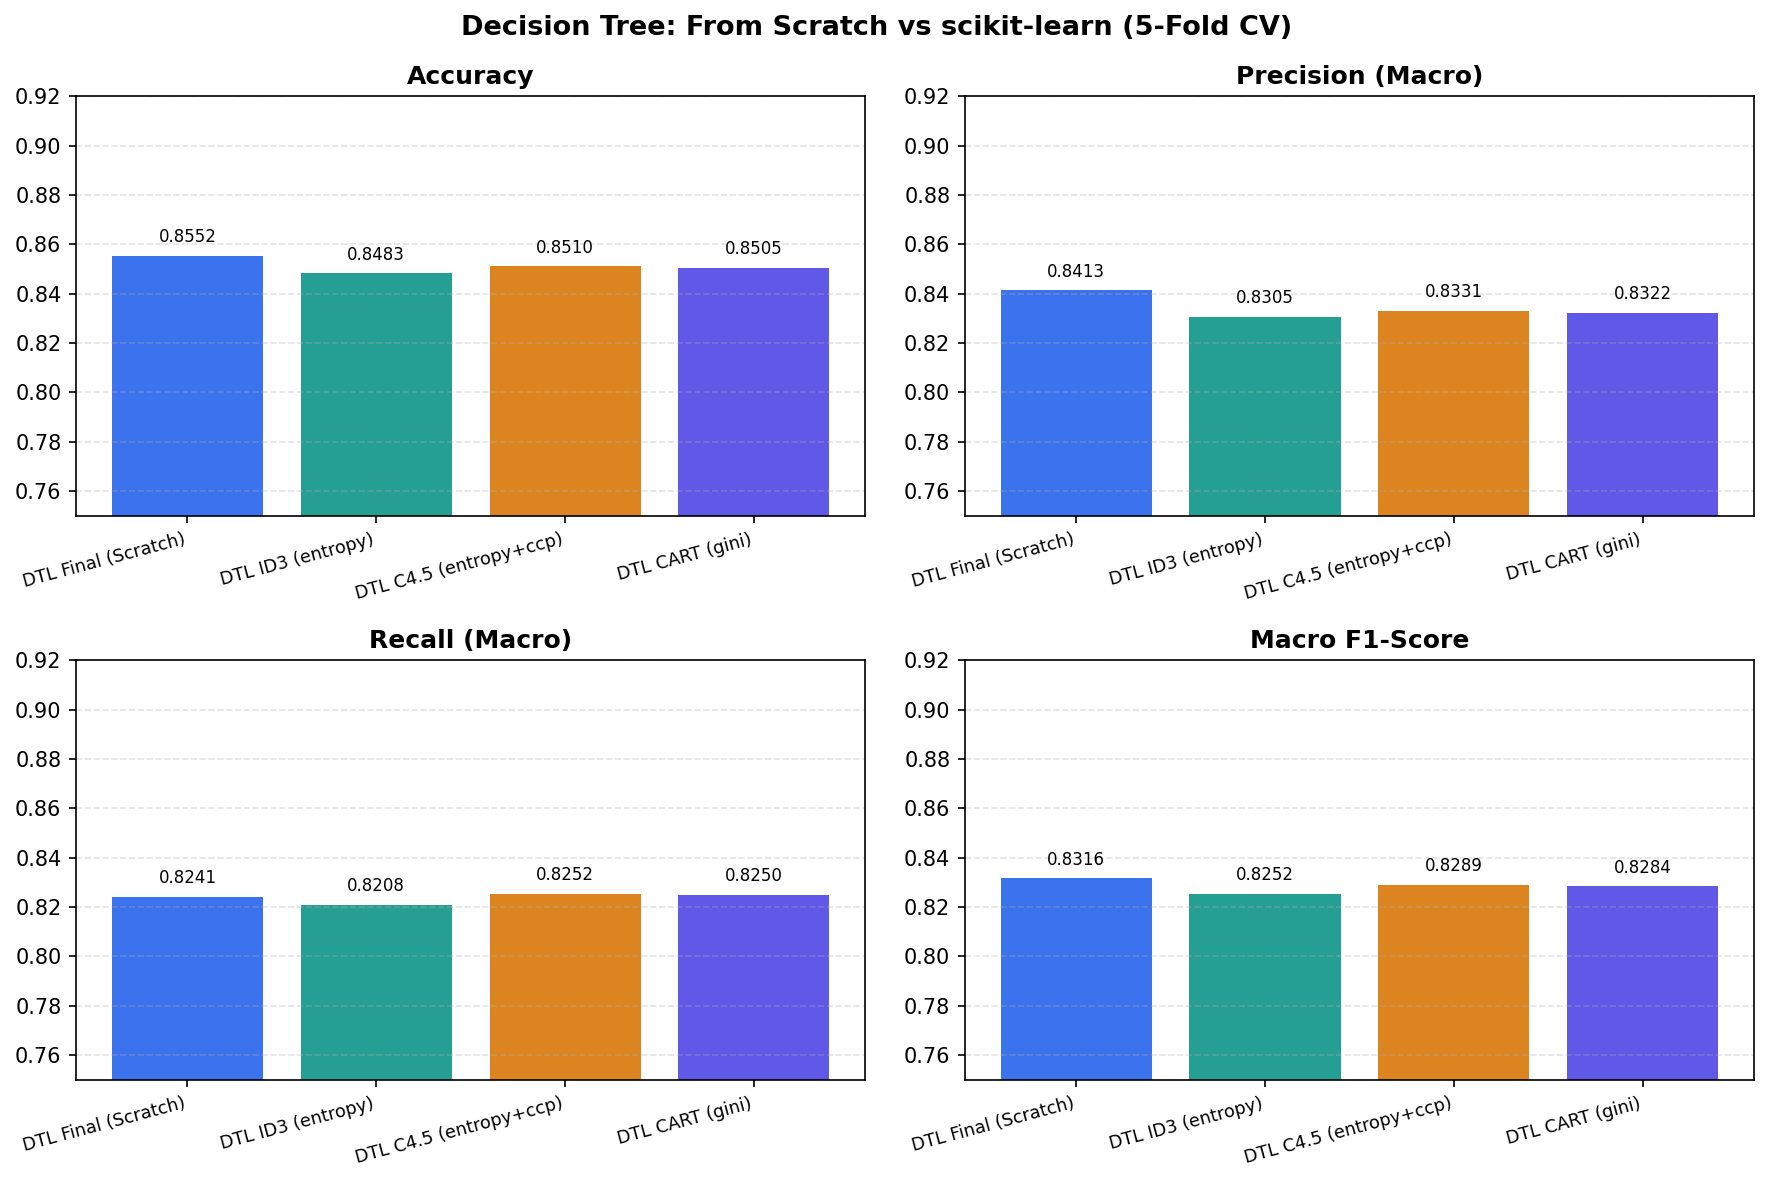
\includegraphics[width=0.92\textwidth]{assets/dtl_vs_sklearn_metrics.png}
  \caption{Perbandingan metrik 5-Fold OOF antara DTL \textit{from scratch} dengan \texttt{scikit-learn} (ID3, C4.5, dan CART).}
  \label{fig:dtl_metrics}
\end{figure}

\begin{figure}[H]
  \centering
  \begin{minipage}[b]{0.48\textwidth}
    \centering
    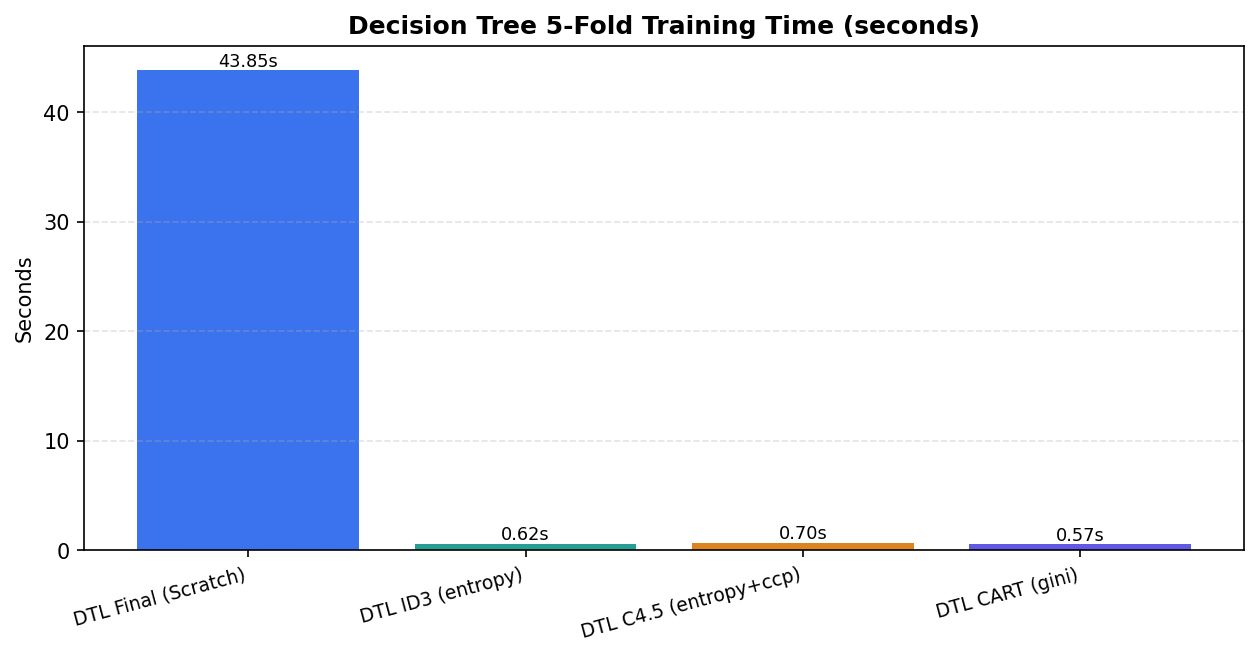
\includegraphics[width=\textwidth]{assets/dtl_vs_sklearn_runtime.png}
    \caption{Perbandingan waktu latih DTL \textit{from scratch} (Python/NumPy) vs \texttt{scikit-learn} (Cython).}
    \label{fig:dtl_rt}
  \end{minipage}
  \hfill
  \begin{minipage}[b]{0.48\textwidth}
    \centering
    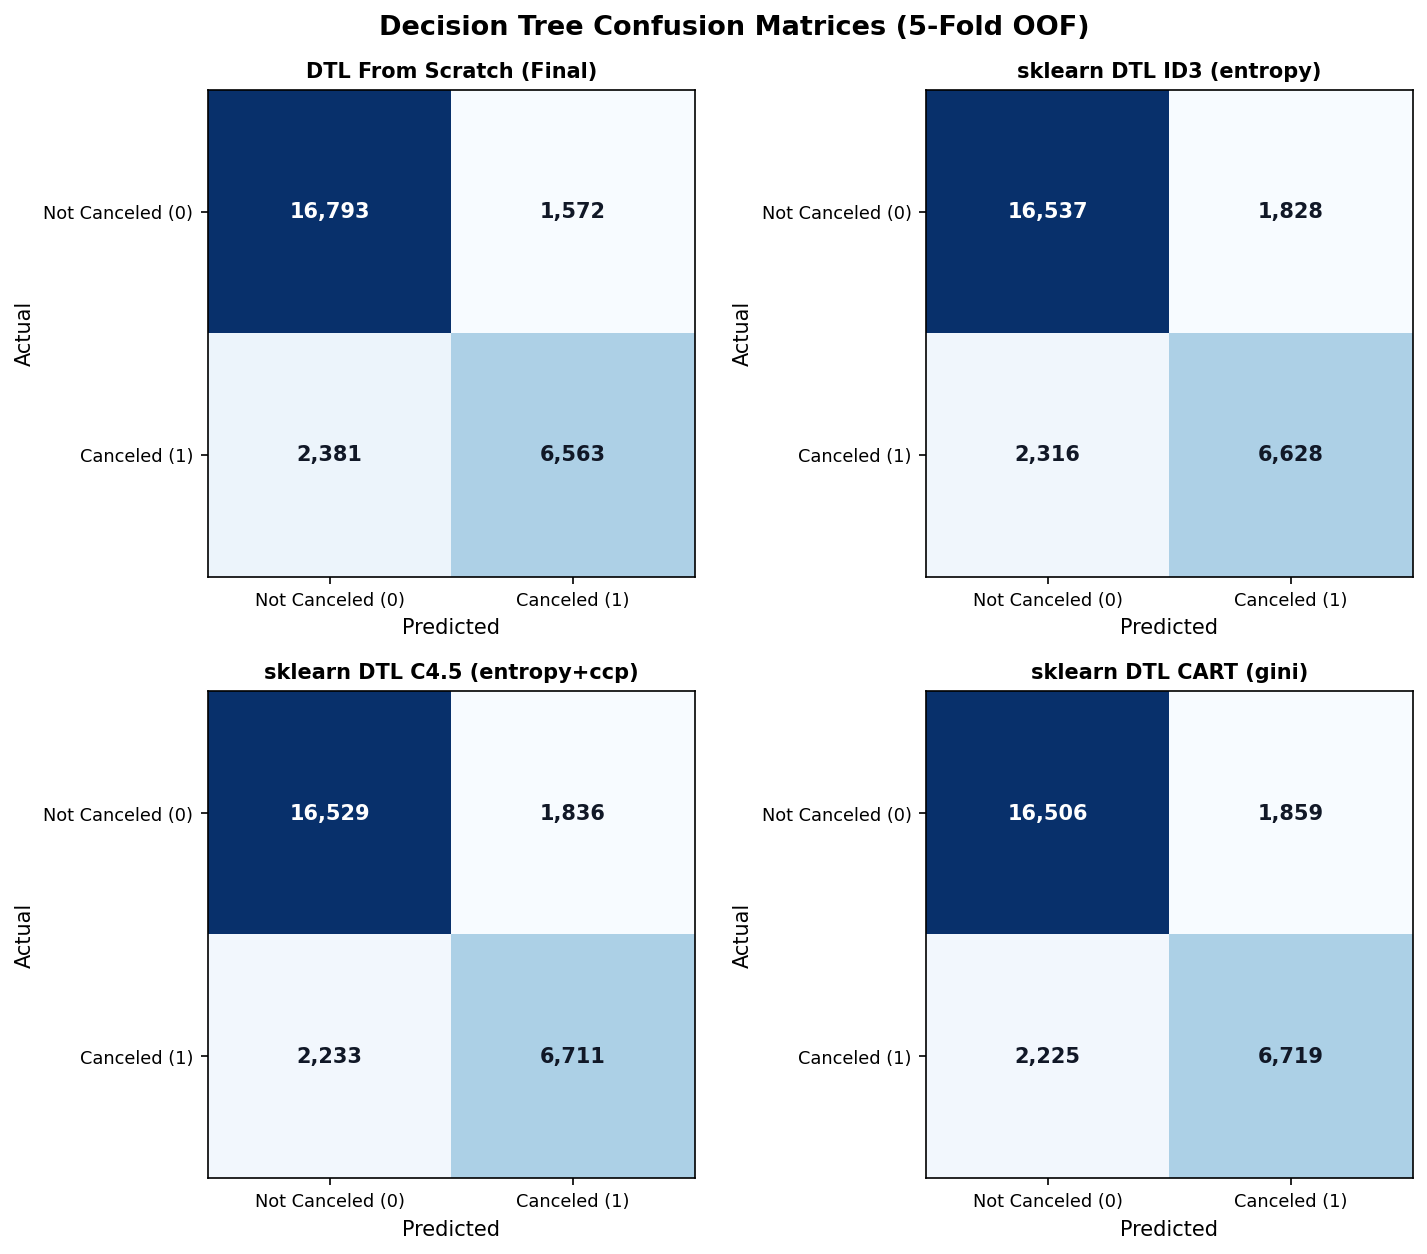
\includegraphics[width=\textwidth]{assets/dtl_confusion_matrices.png}
    \caption{Confusion matrix 5-Fold OOF untuk DTL \textit{from scratch} dan ketiga varian \texttt{scikit-learn}.}
    \label{fig:dtl_cm}
  \end{minipage}
\end{figure}

\subsubsection{Hasil dan Perbandingan Logistic Regression vs \texttt{scikit-learn}}

Pada 59 fitur baseline, keempat mode penalti (\texttt{none}, \texttt{l1}, \texttt{l2}, \texttt{elasticnet}) menunjukkan performa yang sangat dekat dengan \texttt{scikit-learn} (Tabel~\ref{tab:lr}), dengan kesamaan prediksi mencapai \textbf{99,95\%} (\texttt{none}), \textbf{99,91\%} (\texttt{l2}), \textbf{98,36\%} (\texttt{l1}), dan \textbf{98,41\%} (\texttt{elasticnet}). Perbandingan optimizer (Tabel~\ref{tab:lr_opt} dan Gambar~\ref{fig:lr_opt}) membuktikan keunggulan \textbf{L-BFGS} yang mencapai \textit{loss} terendah (0,42608) hanya dalam \textbf{0,21 detik}, sekitar $22\times$ lebih cepat dari SGA (4,63 detik). Dengan penambahan fitur interaksi komposit (982 fitur), Macro F1 melonjak dari 0,7628 menjadi \textbf{0,8609} (kesamaan prediksi \textbf{99,96\%} terhadap \texttt{scikit-learn}). Lintasan parameter $(\theta_0, \theta_1)$ pada kontur \textit{log-loss} ditampilkan pada Gambar~\ref{fig:lr_contour}.

\begin{table}[H]
  \centering
  \small
  \setlength{\tabcolsep}{4pt}
  \caption{Perbandingan Logistic Regression \textit{from scratch} vs \texttt{scikit-learn} pada \texttt{val\_set}.}
  \label{tab:lr}
  \begin{tabularx}{\textwidth}{|Y|L{2.55cm}|R{1.65cm}|R{1.65cm}|R{1.65cm}|R{1.3cm}|}
    \hline
    \rowcolor{tblblue}
    \textbf{Konfigurasi Model} & \textbf{Implementasi} & \textbf{Accuracy} & \textbf{Macro F1} & \textbf{ROC-AUC} & \textbf{Fit (s)} \\
    \hline
    LogReg \texttt{none} (59 fitur) & \texttt{from\_scratch} & 0,8000 & 0,7628 & 0,8597 & 0,23 \\
    \hline
    LogReg \texttt{none} (59 fitur) & \texttt{scikit-learn} & 0,8002 & 0,7629 & 0,8597 & 0,34 \\
    \hline
    LogReg \texttt{l1} (59 fitur) & \texttt{from\_scratch} & 0,7980 & 0,7576 & 0,8592 & 0,86 \\
    \hline
    LogReg \texttt{l1} (59 fitur) & \texttt{scikit-learn} & 0,7998 & 0,7623 & 0,8597 & 6,62 \\
    \hline
    LogReg \texttt{l2} (59 fitur) & \texttt{from\_scratch} & 0,8002 & 0,7627 & 0,8597 & 0,22 \\
    \hline
    LogReg \texttt{l2} (59 fitur) & \texttt{scikit-learn} & 0,8004 & 0,7632 & 0,8597 & 0,21 \\
    \hline
    LogReg \texttt{elasticnet} (59 fitur) & \texttt{from\_scratch} & 0,7978 & 0,7574 & 0,8592 & 0,71 \\
    \hline
    LogReg \texttt{elasticnet} (59 fitur) & \texttt{scikit-learn} & 0,8002 & 0,7628 & 0,8597 & 6,85 \\
    \hline
    \textbf{LogReg Teroptimasi (982 fitur)} & \texttt{from\_scratch} & \textbf{0,8796} & \textbf{0,8609} & \textbf{0,9405} & 1,56 \\
    \hline
    LogReg Teroptimasi (982 fitur) & \texttt{scikit-learn} & 0,8800 & 0,8614 & 0,9405 & 1,01 \\
    \hline
  \end{tabularx}
\end{table}

\begin{table}[H]
  \centering
  \small
  \setlength{\tabcolsep}{4pt}
  \caption{Perbandingan tiga algoritma optimasi pada Logistic Regression L2 baseline (59 fitur).}
  \label{tab:lr_opt}
  \begin{tabularx}{\textwidth}{|Y|R{1.4cm}|R{2.0cm}|R{1.7cm}|R{1.7cm}|R{1.9cm}|}
    \hline
    \rowcolor{tblblue}
    \textbf{Optimizer} & \textbf{Iterasi} & \textbf{Loss Akhir} & \textbf{Accuracy} & \textbf{Macro F1} & \textbf{Fit Time (s)} \\
    \hline
    Stochastic Gradient Ascent & 10 & 0,44142 & 0,7806 & 0,7477 & 4,63 \\
    \hline
    Adam (Bonus) & 60 & 0,42759 & 0,7976 & 0,7572 & 0,59 \\
    \hline
    \textbf{L-BFGS (Bonus)} & 135 & \textbf{0,42608} & \textbf{0,8002} & \textbf{0,7627} & \textbf{0,21} \\
    \hline
  \end{tabularx}
\end{table}

\begin{figure}[H]
  \centering
  \begin{minipage}[b]{0.48\textwidth}
    \centering
    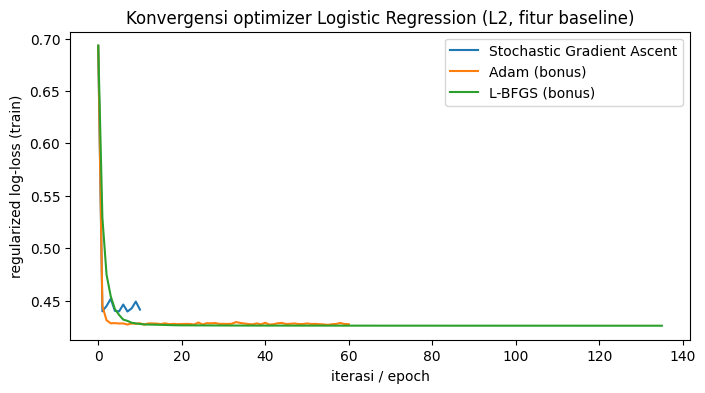
\includegraphics[width=\textwidth]{assets/logreg_optimizers.png}
    \caption{Kurva konvergensi \textit{log-loss} tiga optimizer (SGA, Adam, dan L-BFGS) pada Logistic Regression.}
    \label{fig:lr_opt}
  \end{minipage}
  \hfill
  \begin{minipage}[b]{0.48\textwidth}
    \centering
    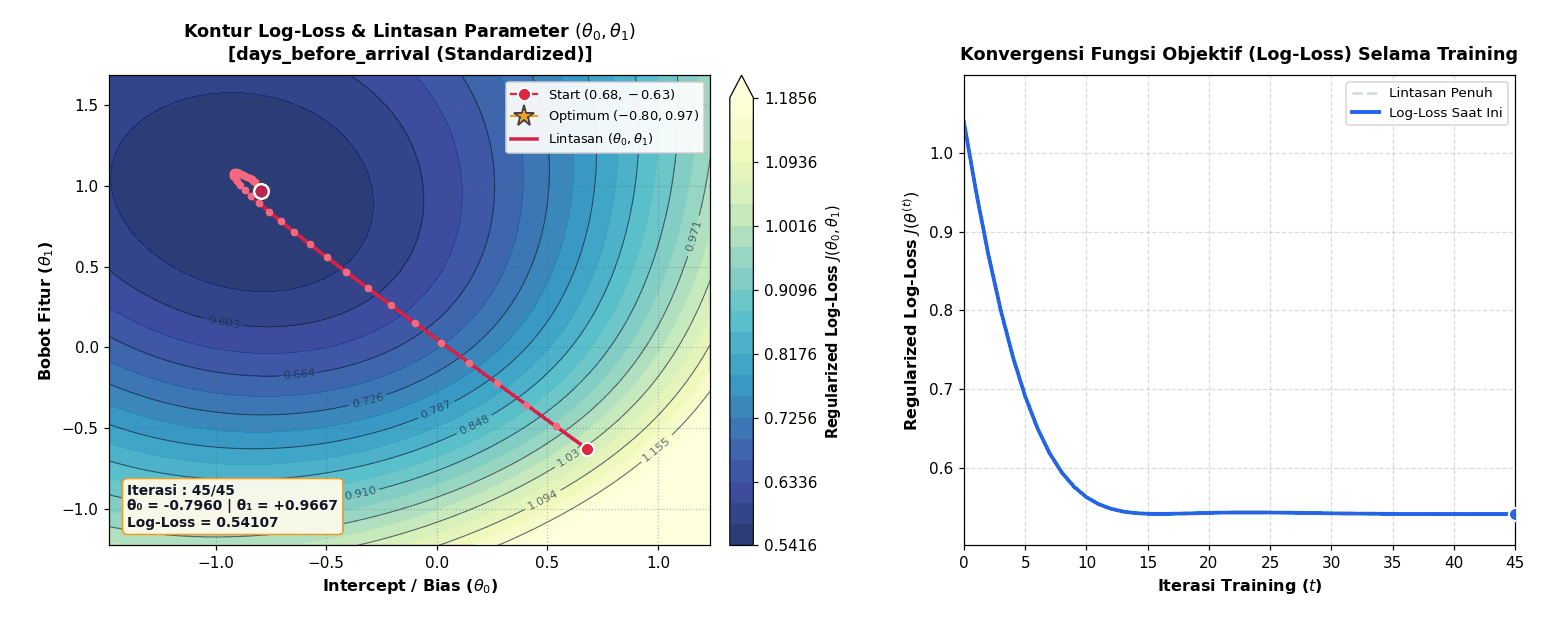
\includegraphics[width=\textwidth]{assets/logreg_contour_frame.png}
    \caption{Bonus visualisasi kontur \textit{log-loss} dan lintasan parameter $(\theta_0, \theta_1)$ (frame akhir \texttt{logreg\_contour.gif}).}
    \label{fig:lr_contour}
  \end{minipage}
\end{figure}

\subsubsection{Hasil dan Perbandingan SVM vs \texttt{scikit-learn}}

Tabel~\ref{tab:svm} menunjukkan bahwa batas keputusan antar kelas pada dataset ini bersifat non-linear: kernel \textbf{Gaussian (RBF)} unggul jauh (Macro F1 \textbf{0,8382}, dan naik menjadi \textbf{0,8393} setelah tuning \textit{threshold} $t=-0{,}30$), diikuti \textbf{Polynomial} (0,8042) dan \textbf{Linear} (0,7628). Perbandingan terhadap \texttt{sklearn.svm.SVC} (LIBSVM) menunjukkan \textbf{kesamaan prediksi 100,00\%} pada Polynomial dan Gaussian serta \textbf{99,98\%} pada Linear, dengan selisih nilai fungsi keputusan maksimum hanya 0,0028 pada Gaussian. Optimasi \textit{shrinking} mempercepat pelatihan Gaussian hingga \textbf{1,44$\times$} (35,09 detik vs 50,49 detik) tanpa mengubah prediksi. Visualisasi 2D bidang pemisah, margin, dan \textit{support vector} ketiga kernel disajikan pada Gambar~\ref{fig:svm_2d} dan~\ref{fig:svm_pca}, serta metrik dan confusion matrix pada Gambar~\ref{fig:svm_met} dan~\ref{fig:svm_cm}.

\begin{table}[H]
  \centering
  \small
  \setlength{\tabcolsep}{3.5pt}
  \caption{Perbandingan 3 kernel SVM \textit{from scratch} vs \texttt{sklearn.svm.SVC} pada \texttt{val\_set} ($t=0$).}
  \label{tab:svm}
  \begin{tabularx}{\textwidth}{|Y|R{1.35cm}|R{1.35cm}|R{1.95cm}|R{1.55cm}|R{1.35cm}|R{1.45cm}|R{1.35cm}|}
    \hline
    \rowcolor{tblblue}
    \textbf{Kernel} & \textbf{F1 Scr.} & \textbf{F1 Sk.} & \textbf{Agreement} & \textbf{Max $|\Delta f|$} & \textbf{n\_SV} & \textbf{Fit Scr.} & \textbf{Fit Sk.} \\
    \hline
    Linear & 0,7628 & 0,7630 & 99,98\% & 0,0346 & 10.274 & 166,05s & 41,32s \\
    \hline
    Polynomial & 0,8042 & 0,8042 & \textbf{100,00\%} & 0,0083 & 8.720 & 32,02s & 16,64s \\
    \hline
    \textbf{Gaussian (RBF)} & \textbf{0,8382} & \textbf{0,8382} & \textbf{100,00\%} & \textbf{0,0028} & 8.077 & 35,09s & 32,36s \\
    \hline
  \end{tabularx}
\end{table}

\begin{figure}[H]
  \centering
  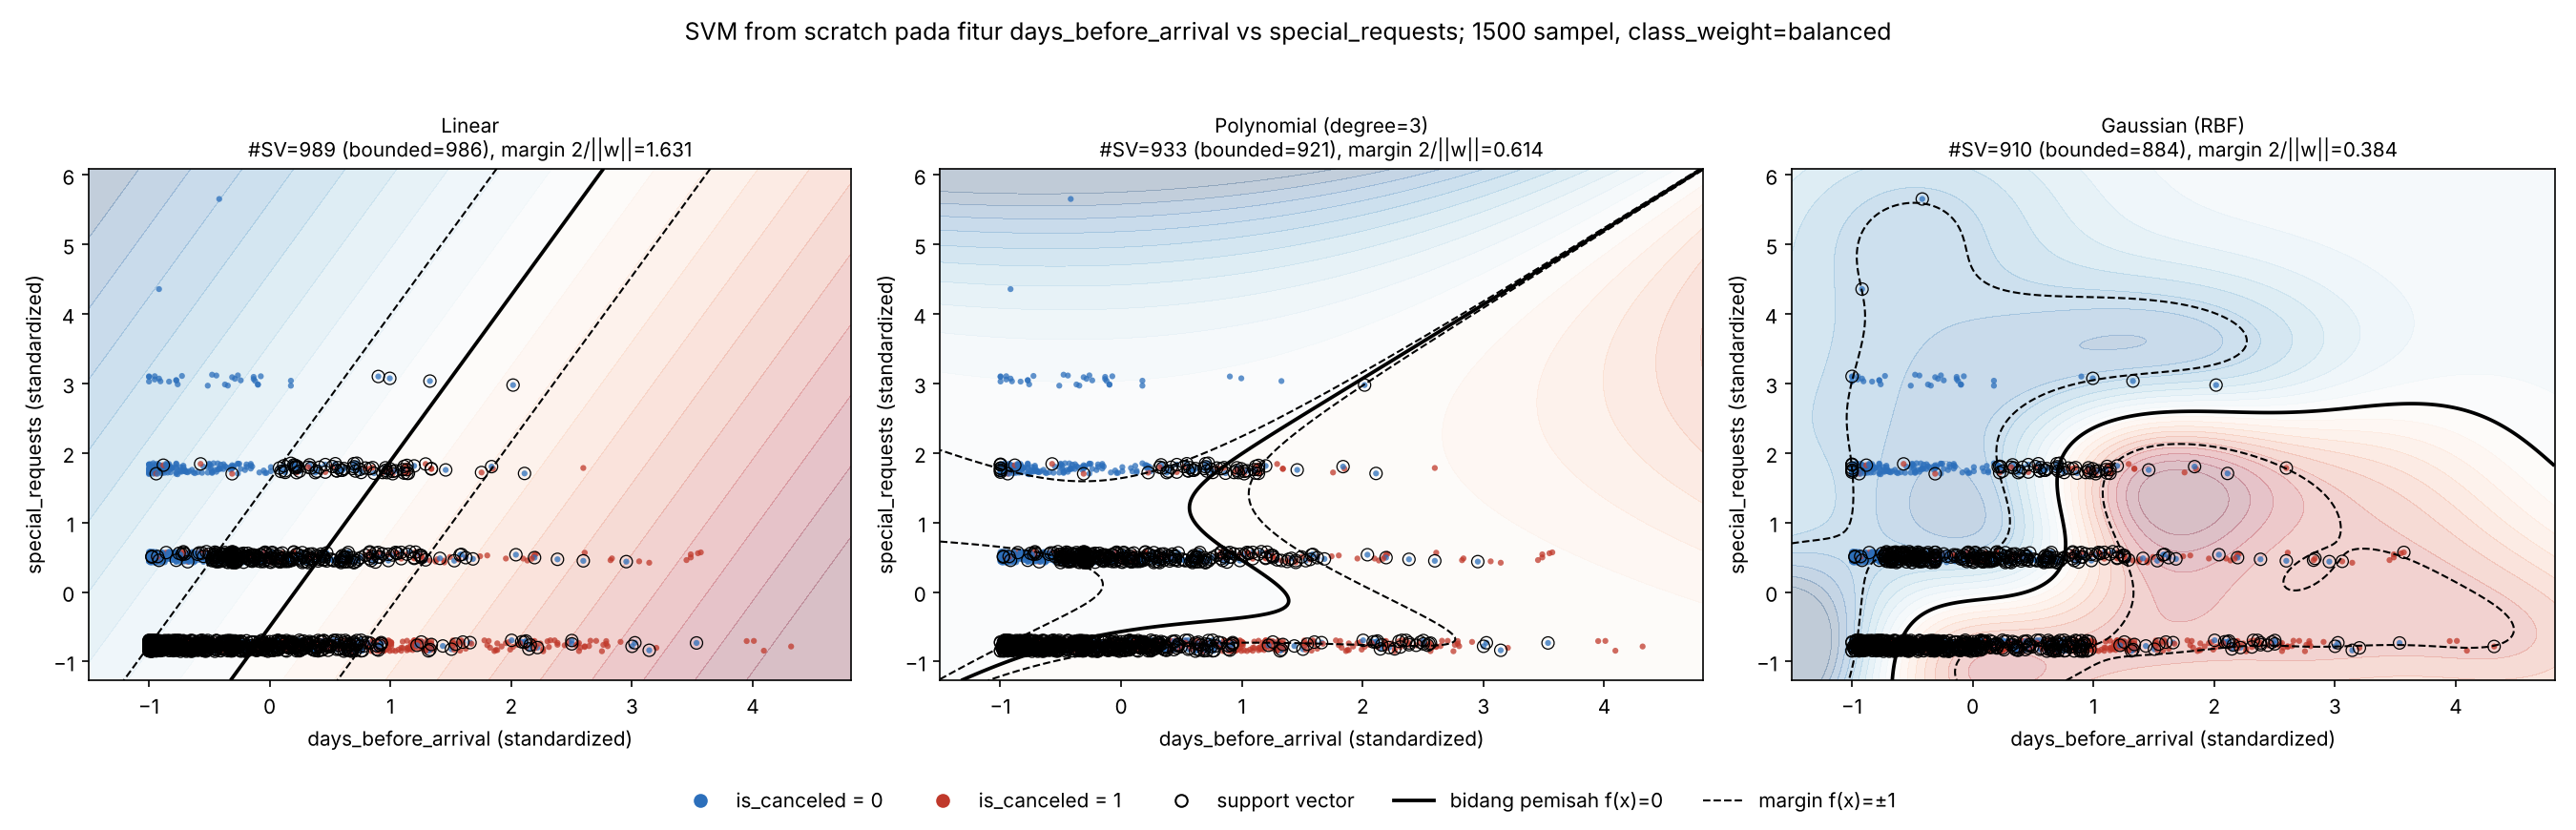
\includegraphics[width=0.96\textwidth]{assets/svm_decision_boundaries.png}
  \caption{Bonus visualisasi 2D bidang pemisah $f(x)=0$, margin $f(x)=\pm 1$, serta \textit{free} dan \textit{bounded support vectors} untuk ketiga kernel SVM pada pasangan fitur (\texttt{days\_before\_arrival}, \texttt{special\_requests}).}
  \label{fig:svm_2d}
\end{figure}

\begin{figure}[H]
  \centering
  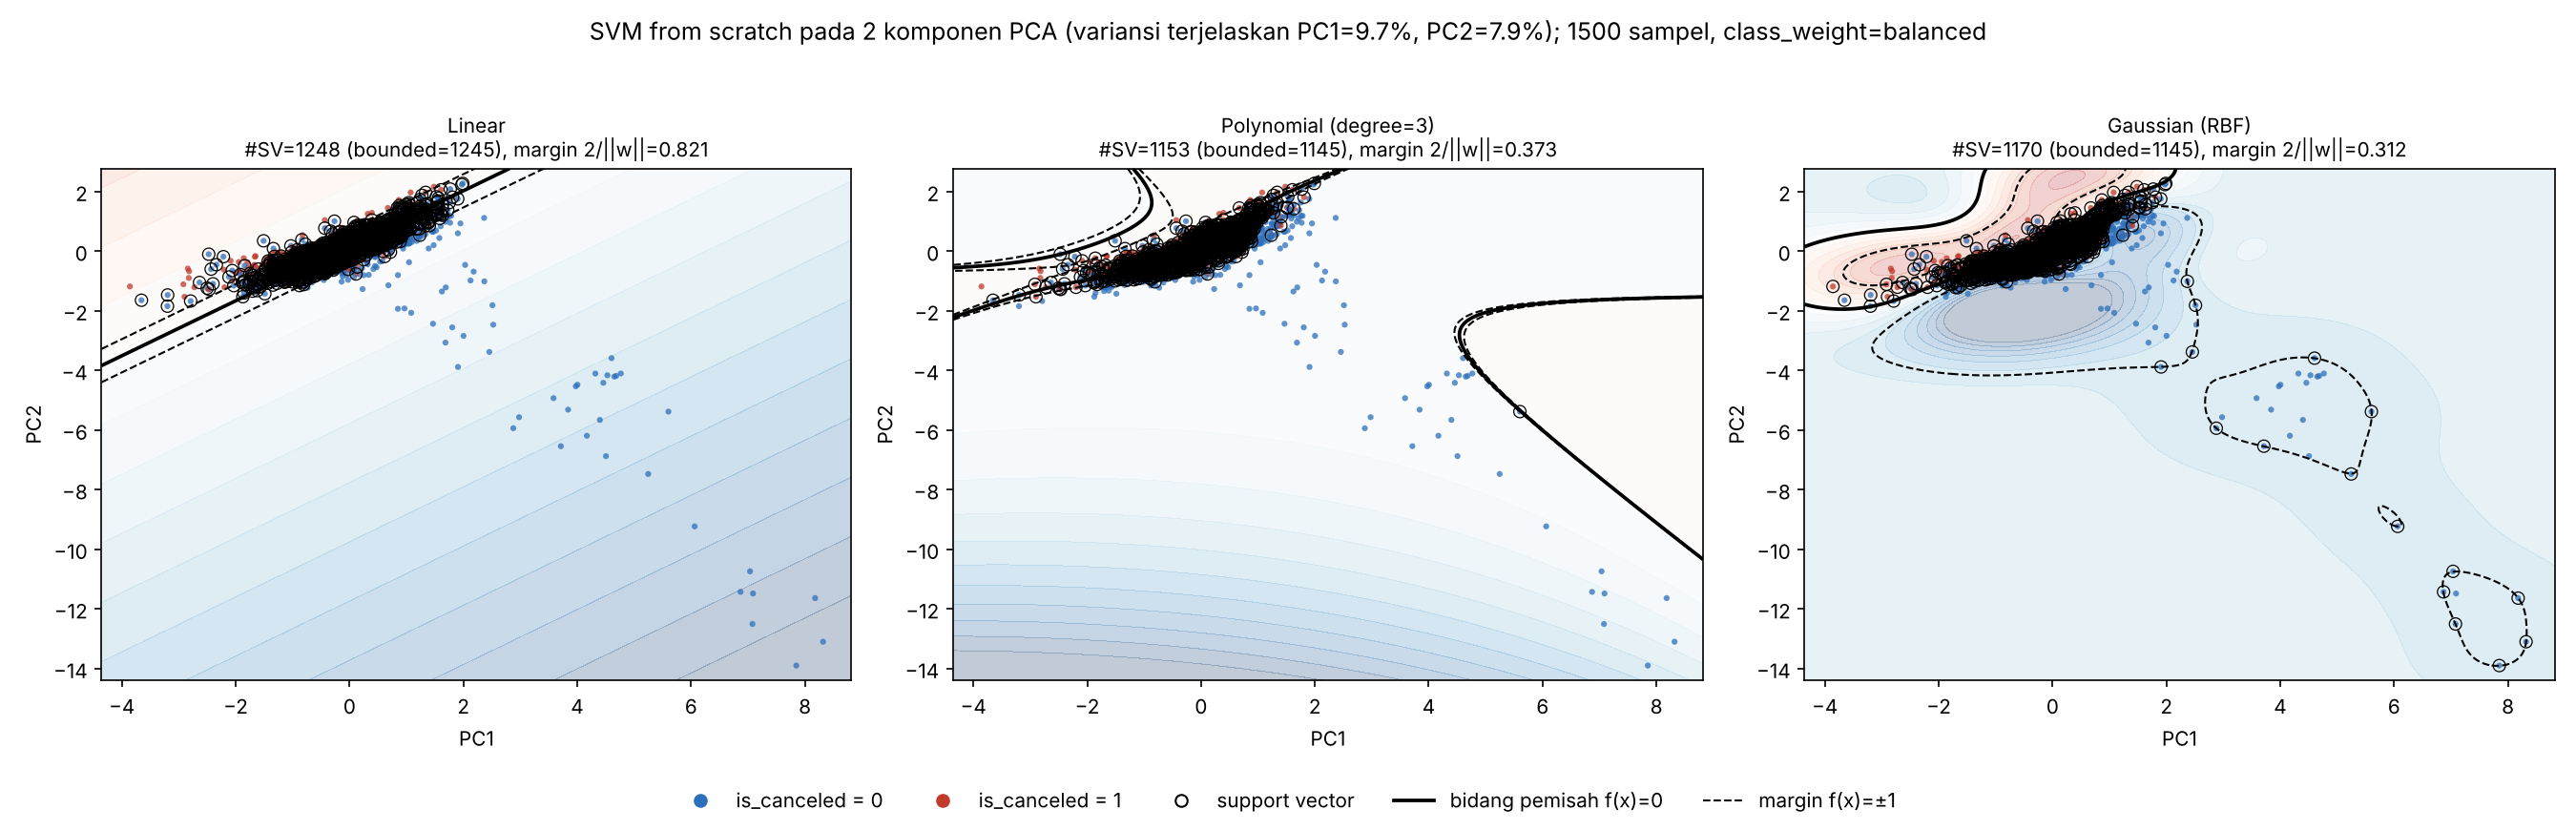
\includegraphics[width=0.96\textwidth]{assets/svm_decision_boundaries_pca.png}
  \caption{Visualisasi 2D bidang pemisah, margin, dan \textit{support vectors} ketiga kernel SVM pada proyeksi 2 komponen utama PCA.}
  \label{fig:svm_pca}
\end{figure}

\clearpage
\begin{figure}[H]
  \centering
  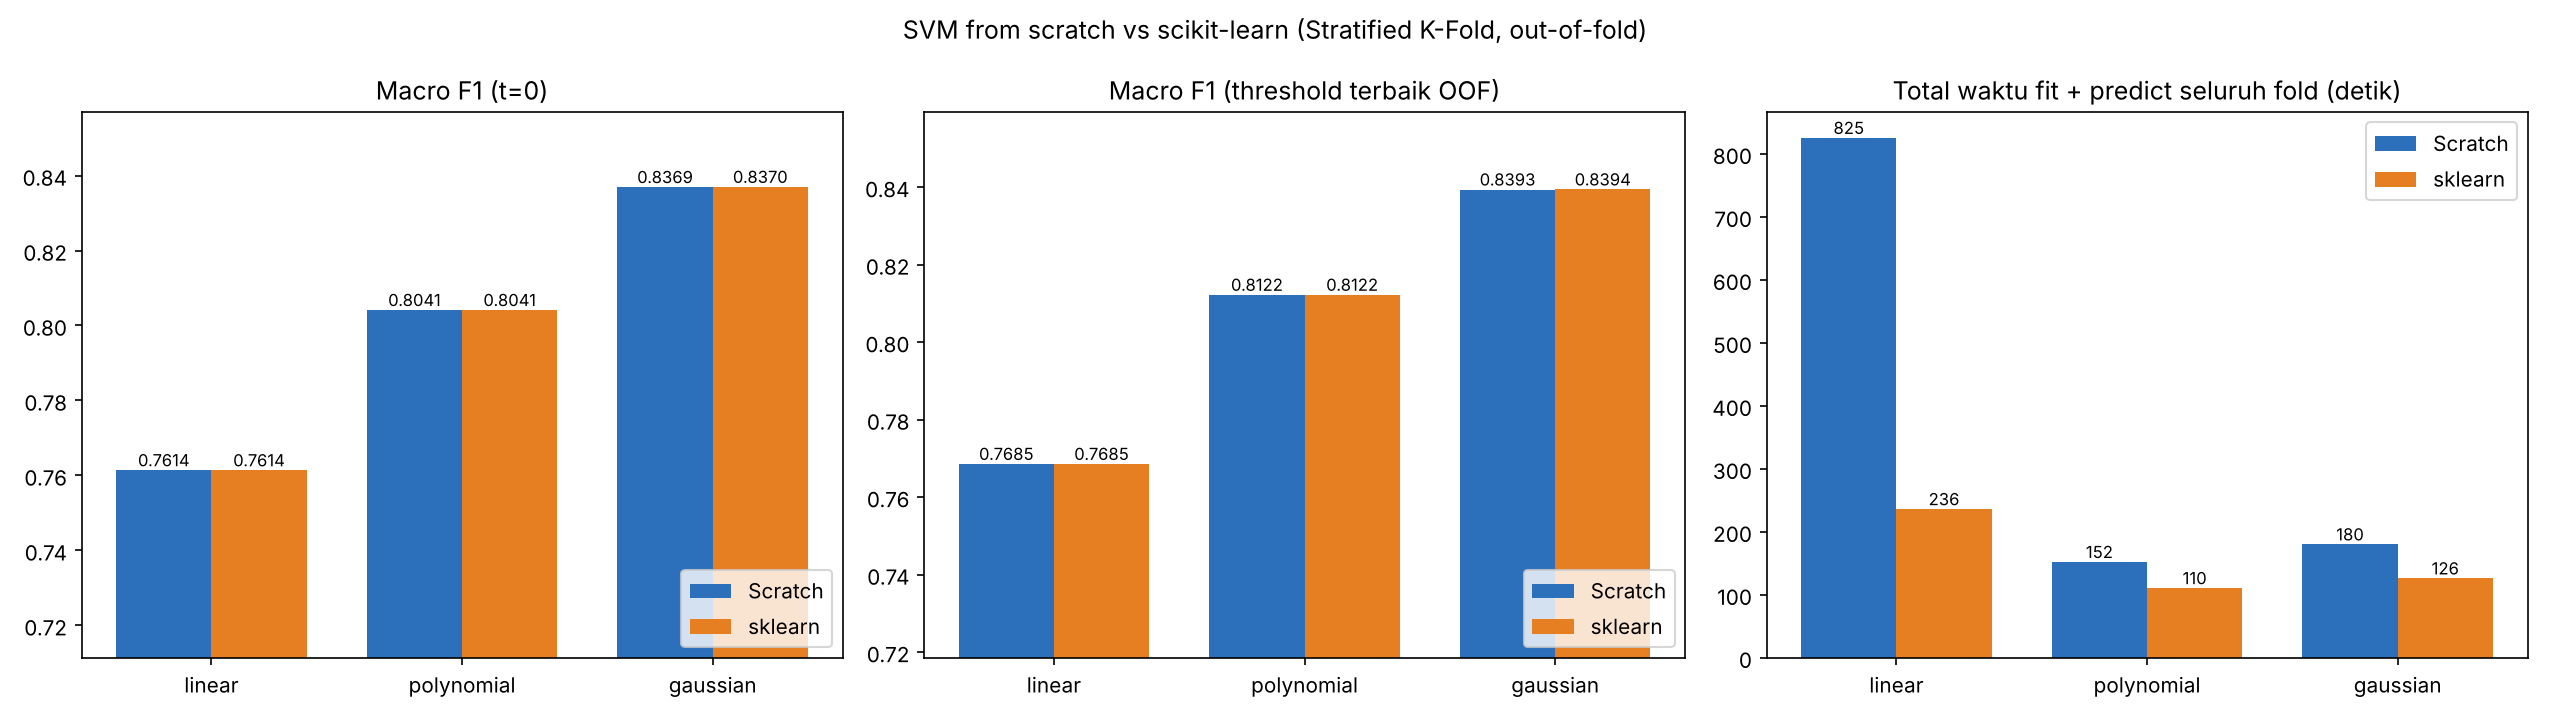
\includegraphics[width=0.92\textwidth]{assets/svm_vs_sklearn_metrics.png}
  \caption{Perbandingan metrik SVM \textit{from scratch} vs \texttt{sklearn.svm.SVC} pada ketiga kernel.}
  \label{fig:svm_met}
\end{figure}

\begin{figure}[H]
  \centering
  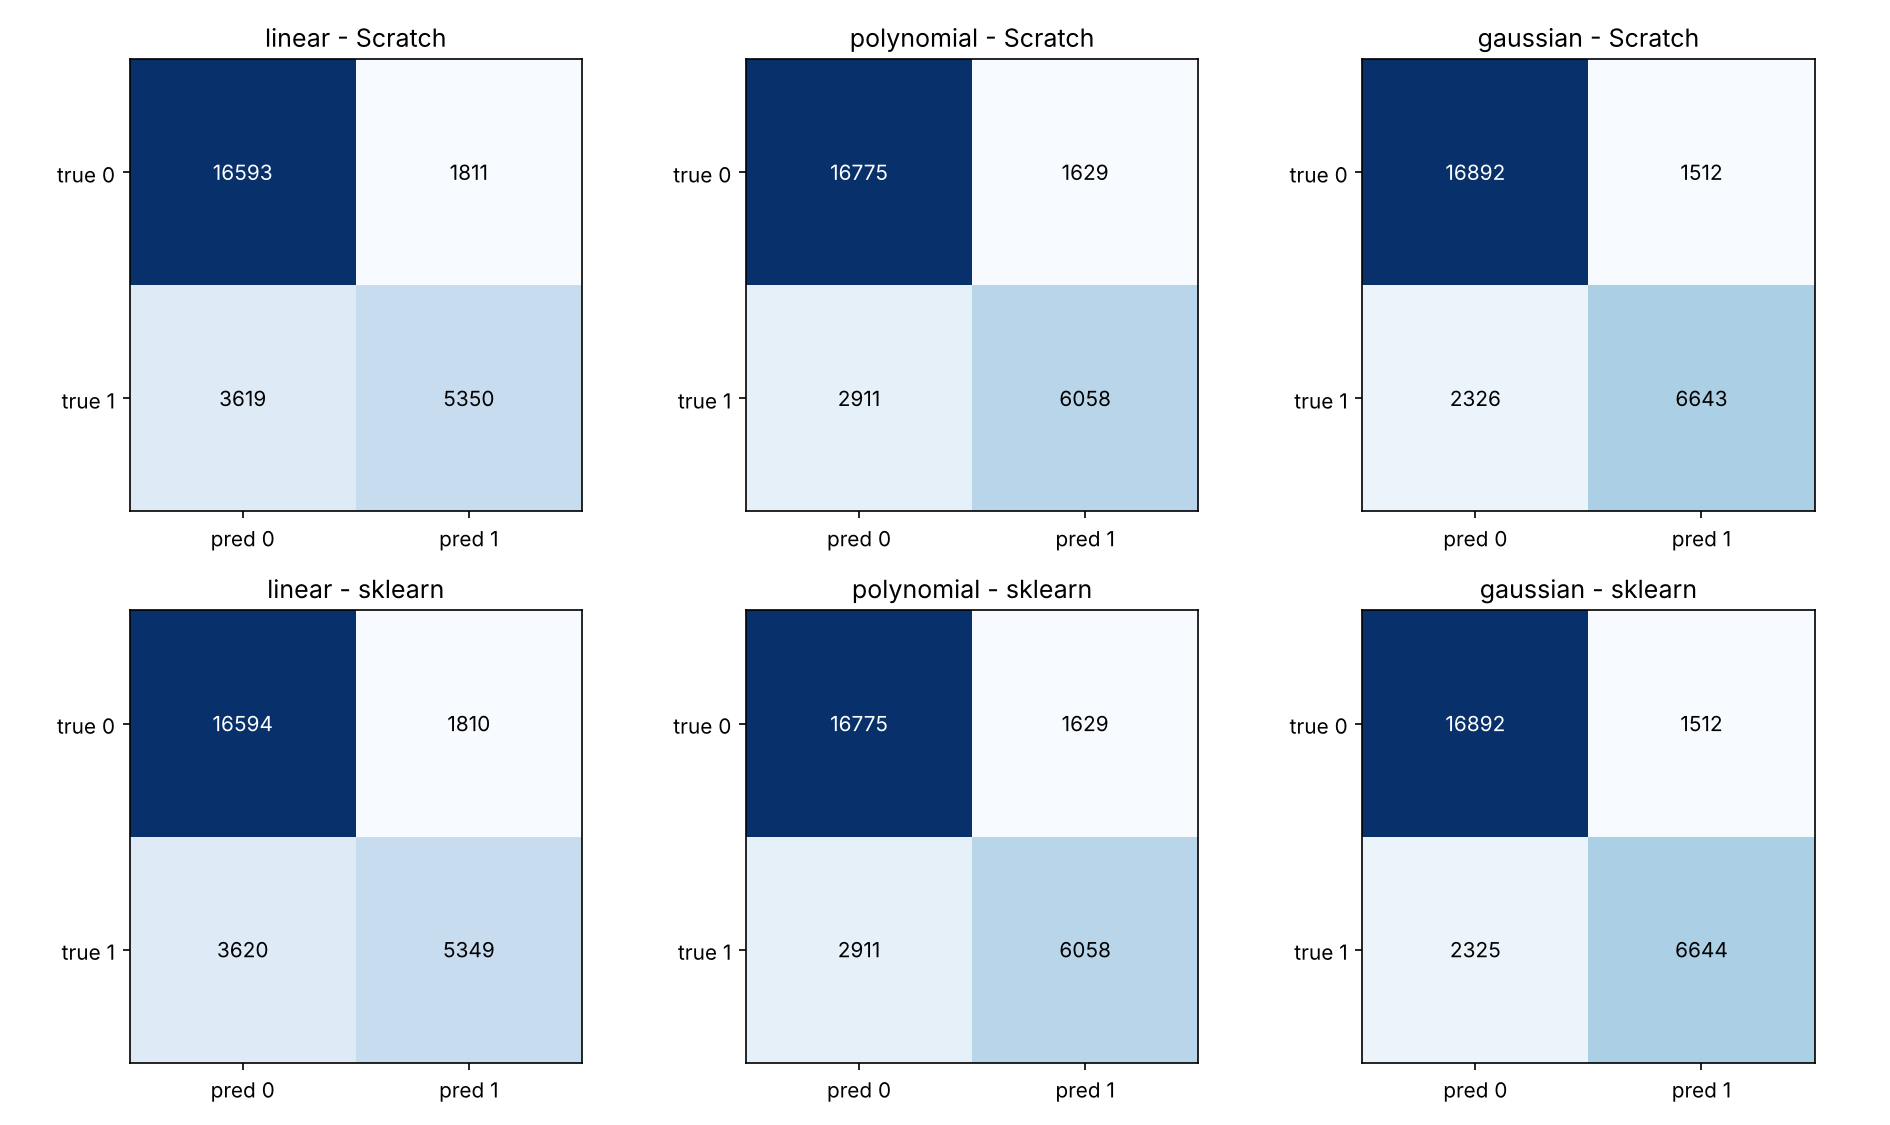
\includegraphics[width=0.92\textwidth]{assets/svm_confusion_matrices.png}
  \caption{Confusion matrix SVM \textit{from scratch} pada ketiga kernel.}
  \label{fig:svm_cm}
\end{figure}

\subsubsection{Hasil dan Perbandingan Naive Bayes vs \texttt{scikit-learn}}

Tabel~\ref{tab:nb} memperlihatkan bahwa asumsi normalitas fitur pada \textbf{Gaussian NB} tidak cocok untuk data campuran yang memuat indikator biner dan distribusi miring (Macro F1 hanya 0,3256, meskipun \textbf{100,00\% identik} dengan \texttt{sklearn.naive\_bayes.GaussianNB}). Diskritisasi fitur pada \textbf{NB Kategorikal (slide)} melompatkan Macro F1 ke 0,7212 (juga \textbf{100,00\% identik} dengan \texttt{CategoricalNB}, selisih probabilitas maksimum $9{,}88 \times 10^{-15}$). Selanjutnya, pelonggaran asumsi independensi bersyarat melalui struktur \textbf{Bayesian Network TAN + CLL} mendorong Macro F1 melonjak ke \textbf{0,8718} (ROC-AUC \textbf{0,9508}), menjadikannya model terbaik di antara seluruh algoritma. Struktur graf berarah Chow-Liu TAN disajikan pada Gambar~\ref{fig:nb_graph}.

\begin{table}[H]
  \centering
  \small
  \setlength{\tabcolsep}{4pt}
  \caption{Perbandingan tiga varian Naive Bayes \textit{from scratch} dan padanan \texttt{scikit-learn} pada \texttt{val\_set}.}
  \label{tab:nb}
  \begin{tabularx}{\textwidth}{|Y|L{2.55cm}|R{1.65cm}|R{1.65cm}|R{1.65cm}|R{1.4cm}|}
    \hline
    \rowcolor{tblblue}
    \textbf{Varian Model} & \textbf{Implementasi} & \textbf{Accuracy} & \textbf{Macro F1} & \textbf{ROC-AUC} & \textbf{Fit (s)} \\
    \hline
    NB Gaussian & \texttt{from\_scratch} & 0,3774 & 0,3256 & 0,8015 & 0,01 \\
    \hline
    NB Gaussian & \texttt{scikit-learn} & 0,3774 & 0,3256 & 0,8015 & 0,01 \\
    \hline
    NB Kategorikal (slide) & \texttt{from\_scratch} & 0,7485 & 0,7212 & 0,8142 & 0,81 \\
    \hline
    NB Kategorikal (slide) & \texttt{scikit-learn} & 0,7485 & 0,7212 & 0,8142 & 0,02 \\
    \hline
    \textbf{NB TAN + CLL (Bonus)} & \texttt{from\_scratch} & \textbf{0,8895} & \textbf{0,8718} & \textbf{0,9508} & 233,33 \\
    \hline
  \end{tabularx}
\end{table}

\begin{figure}[H]
  \centering
  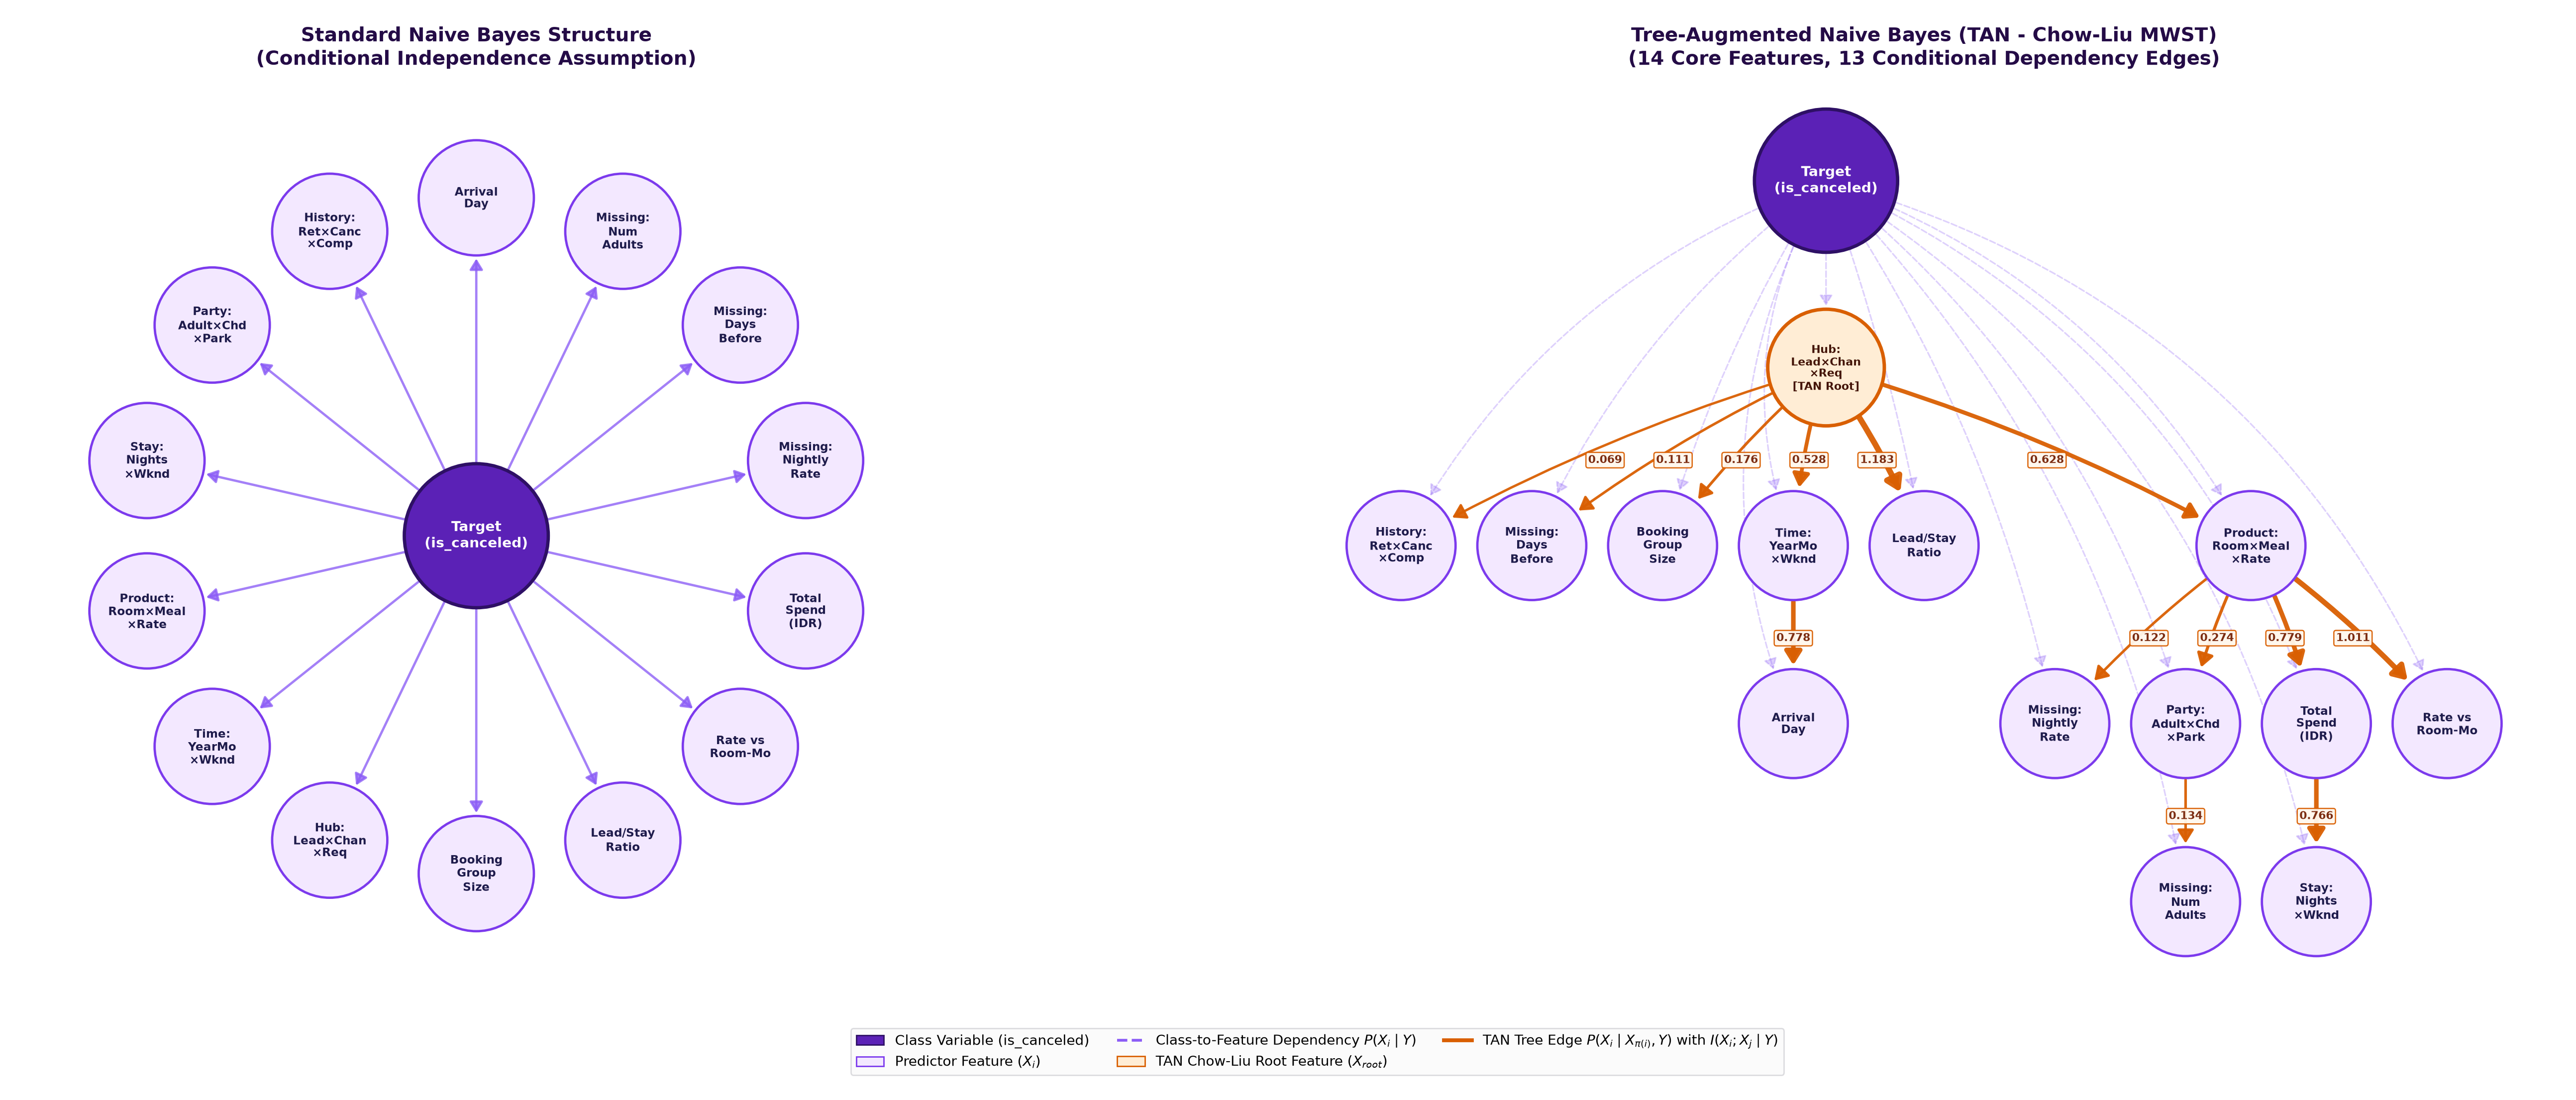
\includegraphics[width=0.95\textwidth]{assets/naive_bayes_graph.png}
  \caption{Bonus visualisasi graf berarah Bayesian Network (TAN Chow-Liu): simpul target \texttt{is\_canceled} menjadi induk seluruh fitur, dan setiap fitur terhubung ke paling banyak satu induk fitur berdasarkan CMI tertinggi.}
  \label{fig:nb_graph}
\end{figure}

\subsubsection{Bonus: Analisis \textit{Cost-Sensitive Classification} ($C_{\text{FP}} = 2 \cdot C_{\text{FN}}$)}

Pada skenario bisnis di mana biaya \textit{False Positive} (kamar dijual ulang lalu terjadi \textit{overbooking}) bernilai dua kali lipat dari biaya \textit{False Negative} (kamar terlanjur kosong), fungsi biaya total didefinisikan sebagai $\text{Cost} = 2 \cdot \text{FP} + 1 \cdot \text{FN}$. Berdasarkan teorema keputusan Bayes\fnmark{19}, ambang probabilitas optimal teoretis adalah:
\[
  \tau^* = \frac{C_{\text{FP}}}{C_{\text{FP}} + C_{\text{FN}}} = \frac{2}{2 + 1} = \frac{2}{3} \approx 0{,}667.
\]
Eksperimen dijalankan pada model SVM Gaussian dengan tiga pendekatan: (1) \textit{Bayes threshold} melalui kalibrasi Platt ($A=-1{,}705, B=0{,}129$, setara $f(x) \ge 0{,}482$), (2) \textit{tuned threshold} berbasis biaya OOF ($f(x) \ge 0{,}460$), dan (3) \textit{cost-weighted training} dengan bobot penalti kelas negatif $C_0 = 2C$. Hasil pada Tabel~\ref{tab:cost} dan Gambar~\ref{fig:cost} menunjukkan bahwa ketiga strategi berhasil \textbf{menekan total biaya sebesar 17,1\%--17,9\%} (dari 1.173 turun menjadi 963--972) dengan memotong jumlah FP lebih dari separuh (396 $\rightarrow$ 138--174).

\begin{table}[H]
  \centering
  \small
  \setlength{\tabcolsep}{4pt}
  \caption{Hasil evaluasi \textit{Cost-Sensitive Classification} ($C_{\text{FP}} = 2, C_{\text{FN}} = 1$) pada \texttt{val\_set}.}
  \label{tab:cost}
  \begin{tabularx}{\textwidth}{|Y|R{1.45cm}|R{1.05cm}|R{1.05cm}|R{1.3cm}|R{1.55cm}|R{1.95cm}|}
    \hline
    \rowcolor{tblblue}
    \textbf{Strategi} & \textbf{Thr. $f$} & \textbf{FP} & \textbf{FN} & \textbf{Biaya} & \textbf{Macro F1} & \textbf{Penurunan} \\
    \hline
    Baseline ($t$ Macro F1) & $-0{,}300$ & 396 & 381 & 1.173 & \textbf{0,8393} & 0,0\% \\
    \hline
    Bayes Threshold (Platt, $p \ge 2/3$) & $0{,}482$ & 171 & 626 & 968 & 0,8218 & $-17{,}5\%$ \\
    \hline
    Tuned Threshold (biaya OOF) & $0{,}460$ & 174 & 624 & 972 & 0,8218 & $-17{,}1\%$ \\
    \hline
    \textbf{Cost-Weighted Training ($C_0=2C$)} & $0{,}000$ & \textbf{138} & 687 & \textbf{963} & 0,8121 & \textbf{$-17{,}9\%$} \\
    \hline
  \end{tabularx}
\end{table}

\begin{figure}[H]
  \centering
  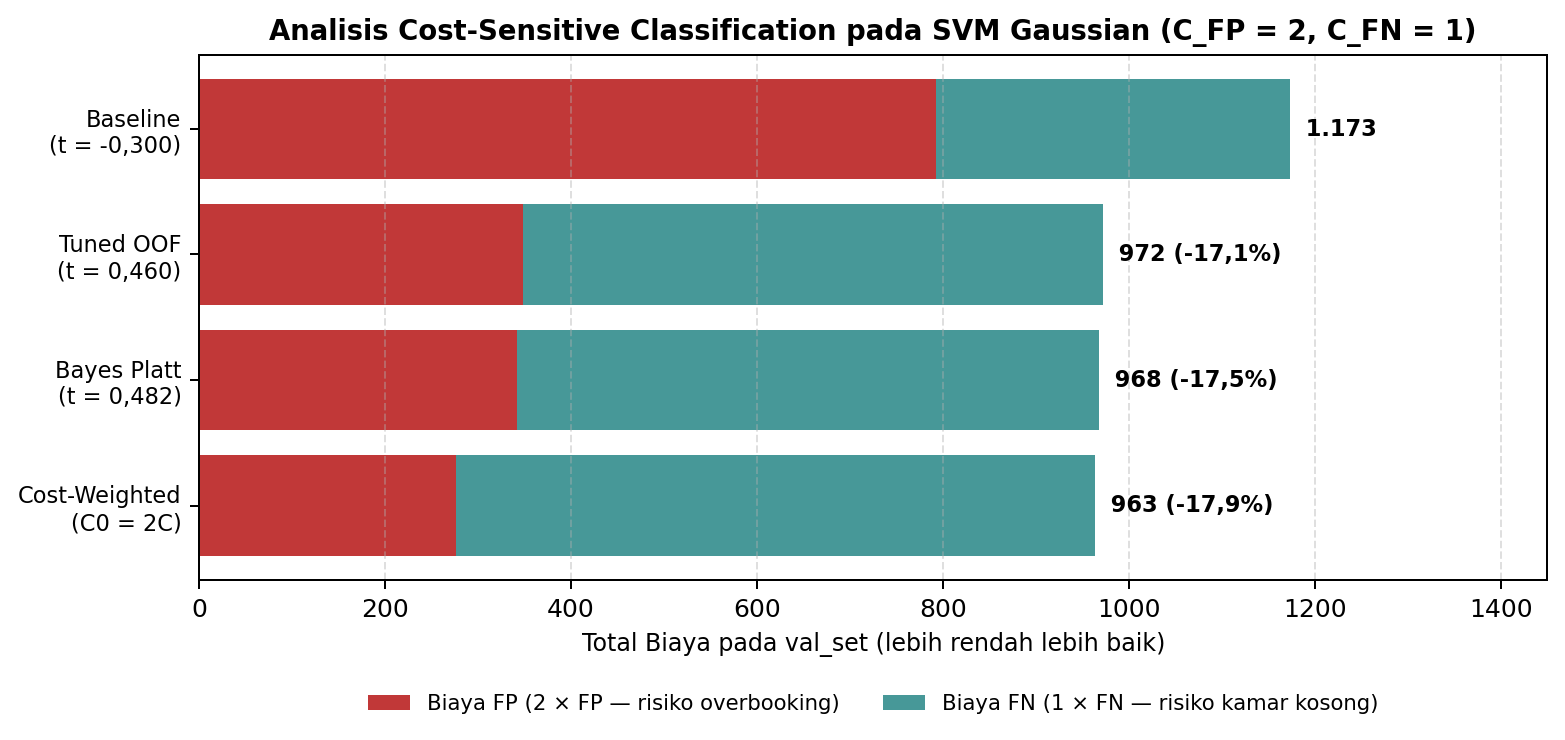
\includegraphics[width=0.84\textwidth]{assets/cost_sensitive_comparison.png}
  \caption{Perbandingan komposisi biaya ($2\cdot\text{FP}$ dan $1\cdot\text{FN}$) antar strategi \textit{cost-sensitive} pada \texttt{val\_set}.}
  \label{fig:cost}
\end{figure}

\clearpage
\subsubsection{Verifikasi \textit{Save \& Load} dan \textit{Error Analysis}}

Seluruh 5 model final yang dilatih pada data penuh berhasil disimpan ke \texttt{output/models/*.pkl} dan dimuat kembali dengan \textbf{prediksi serta probabilitas 100\% identik} sebelum dan sesudah \textit{reload} (Tabel~\ref{tab:saveload}).

\begin{table}[H]
  \centering
  \small
  \setlength{\tabcolsep}{5pt}
  \caption{Hasil verifikasi serialisasi \textit{save} dan \textit{load} seluruh lima model final.}
  \label{tab:saveload}
  \begin{tabularx}{\textwidth}{|L{3.4cm}|>{\raggedright\arraybackslash\footnotesize}X|R{1.9cm}|C{2.4cm}|}
    \hline
    \rowcolor{tblblue}
    \textbf{Model} & \textbf{Berkas Tersimpan} & \textbf{Ukuran} & \textbf{Reload Identik} \\
    \hline
    Naive Bayes TAN+CLL & \path{output/models/naive_bayes_model_v6.pkl} & 69,40 MB & Ya (100\%) \\
    \hline
    KNN Berbobot Fitur & \path{output/models/knn_kaggle.pkl} & 10,49 MB & Ya (100\%) \\
    \hline
    SVM Gaussian & \path{output/models/svm_kaggle.pkl} & 5,09 MB & Ya (100\%) \\
    \hline
    DTL CART & \path{output/models/dtl_kaggle.pkl} & 0,30 MB & Ya (100\%) \\
    \hline
    Logistic Regression & \path{output/models/logreg_kaggle.pkl} & 0,01 MB & Ya (100\%) \\
    \hline
  \end{tabularx}
\end{table}

Berdasarkan \textit{error analysis} pada \texttt{val\_set} (5.475 baris), sebanyak \textbf{4.364 baris (79,7\%)} diprediksi benar secara serentak oleh model-model utama, sementara \textbf{363 baris (6,6\%)} salah diprediksi oleh seluruh model secara bersamaan (menandakan adanya \textit{irreducible noise} dari faktor eksternal di luar fitur dataset). Segmen dengan tingkat kesalahan terbesar terkonsentrasi pada kanal \textbf{Online Travel Agent} (\textit{error rate} 15,9\%, 3.519 baris), rentang waktu tunggu menengah \textbf{31--180 hari} (\textit{error rate} 15,1\%), serta pemesanan dengan \texttt{special\_requests} kosong (\textit{error rate} 14,6\%).

% =====================================================================
% BAB 3: KESIMPULAN DAN SARAN
% =====================================================================
\clearpage
\section{Kesimpulan dan Saran}

\subsection{Kesimpulan}

\begin{enumerate}[leftmargin=1.4cm, itemsep=3pt]
  \item Seluruh tahapan pengolahan data (\textit{cleaning}, imputasi dengan indikator nilai kosong, rekayasa fitur domain, \textit{encoding}, \textit{scaling}, seleksi fitur mRMR, serta evaluasi PCA dan \textit{resampling}) telah diimplementasikan secara terpisah pada data latih dan uji tanpa \textit{data leakage}. Hasil eksperimen membuktikan bahwa mempertahankan seluruh fitur tanpa PCA dan tanpa \textit{resampling} (diganti \textit{threshold tuning}) memberikan Macro F1 terbaik.
  \item Kelima algoritma \textit{supervised learning} (\textbf{KNN}, \textbf{DTL CART}, \textbf{Logistic Regression} dengan L1/L2/Elastic Net, \textbf{SVM} dengan kernel Linear/Polynomial/Gaussian, dan \textbf{Bayesian Network / Naive Bayes}) berhasil diimplementasikan 100\% \textit{from scratch} dengan \texttt{NumPy} dan pustaka standar Python, serta mencapai kesesuaian prediksi \textbf{98,4\%--100,0\%} terhadap padanan \texttt{scikit-learn}.
  \item Model tunggal terbaik adalah \textbf{Naive Bayes TAN + CLL} dengan Macro F1 validasi \textbf{0,8718} (ROC-AUC \textbf{0,9508}) dan skor Kaggle Public Leaderboard \textbf{0,87066}, diikuti oleh Logistic Regression teroptimasi (\textbf{0,86410}), KNN berbobot fitur (\textbf{0,85633}), SVM Gaussian (\textbf{0,85254}), dan DTL CART (\textbf{0,84226}).
  \item Seluruh mekanisme optimasi dan visualisasi bonus (\textit{Minimal Cost-Complexity Pruning}, \texttt{plot\_tree}, Adam \& L-BFGS, animasi kontur \textit{log-loss}, SMO+WSS2+\textit{shrinking}, bidang pemisah 2D SVM, graf Chow-Liu TAN, serta \textit{Cost-Sensitive Classification} $C_{\text{FP}}=2C_{\text{FN}}$ yang memangkas biaya hingga \textbf{17,9\%}) berhasil diterapkan dan diverifikasi.
\end{enumerate}

\subsection{Saran}

\begin{enumerate}[leftmargin=1.4cm, itemsep=3pt]
  \item \textbf{Akselerasi Komputasi}: Pada DTL, SVM, dan Naive Bayes TAN+CLL, waktu pelatihan \textit{from scratch} berbasis Python masih jauh lebih lambat dibanding pustaka berbahasa C/Cython (\texttt{scikit-learn}). Pemanfaatan vektorisasi matriks yang lebih dalam atau kompilasi numerik (seperti Cython/Numba pada eksperimen produksi) dapat mempercepat eksperimen secara signifikan.
  \item \textbf{Eksplorasi Fitur Eksternal}: Karena 6,6\% data validasi salah diprediksi oleh seluruh model sekaligus (khususnya pada kanal \textit{Online Travel Agent} dan waktu tunggu 31--180 hari), penambahan sinyal eksternal seperti kebijakan pembatalan (\textit{refundable} vs \textit{non-refundable}), jenis pembayaran/deposit, dan kalender hari libur berpotensi menekan tingkat kesalahan lebih lanjut.
  \item \textbf{Kalibrasi Probabilitas Lintas Model}: Untuk penerapan bisnis berbasis \textit{cost-sensitive}, kalibrasi probabilitas (seperti \textit{Platt scaling} atau \textit{isotonic regression}) sebaiknya dievaluasi pula pada Naive Bayes TAN+CLL dan Logistic Regression agar penentuan ambang $\tau^*$ semakin presisi.
\end{enumerate}

% =====================================================================
% BAB 4: LAMPIRAN
% =====================================================================
\clearpage
\section{Lampiran}

\subsection{Detail Pembagian Tugas}

Tabel~\ref{tab:pembagian} merangkum pembagian kontribusi dari kelima anggota Kelompok 09 -- Aduhmen.

\begin{table}[H]
  \centering
  \small
  \setlength{\tabcolsep}{5pt}
  \caption{Detail pembagian tugas anggota Kelompok 09 -- Aduhmen.}
  \label{tab:pembagian}
  \begin{tabularx}{\textwidth}{|L{4.8cm}|Y|}
    \hline
    \rowcolor{tblblue}
    \textbf{Nama Penanggung Jawab (NIM)} & \textbf{Detail Tugas} \\
    \hline
    Ardell Aghna Mahendra (13523151) & Implementasi Logistic Regression (L1, L2, Elastic Net, SGA/Adam/L-BFGS, animasi kontur log-loss), penyusunan dan audit reproduksibilitas notebook, penyusunan laporan. \\
    \hline
    Fazri Arrashyi Putra (13524127) & Implementasi K-Nearest Neighbors (KNN + pembobotan fitur), EDA dan preprocessing dasar, integrasi notebook, penyusunan laporan. \\
    \hline
    Dika Pramudya Nugraha (13524132) & Implementasi Bayesian Network / Naive Bayes (Gaussian, Kategorikal, TAN Chow-Liu + CLL + visualisasi graf), modul \texttt{preprocessing.py}, \texttt{README.md}, penyusunan laporan. \\
    \hline
    Daniel Putra Rywandi S. (13524143) & Implementasi Support Vector Machine (Linear, Polynomial, Gaussian, SMO + WSS2 + shrinking, visualisasi 2D), modul \texttt{metrics.py}, analisis \textit{Cost-Sensitive}, penyusunan laporan. \\
    \hline
    Dzakwan Muhammad Khairan Putra Purnama (13524145) & Implementasi Decision Tree Learning (CART/Entropy, native null handling, Minimal Cost-Complexity Pruning, \texttt{plot\_tree}), modul \texttt{model\_io.py}, finalisasi dan eksekusi notebook, perancangan dan penyusunan laporan LaTeX. \\
    \hline
  \end{tabularx}
\end{table}

\subsection{Lampiran Lainnya}

\begin{itemize}[leftmargin=1.2cm, itemsep=3pt]
  \item \textbf{Repository GitHub}: \url{https://github.com/fazridep/IF3170_G09_Aduhmen}
  \item \textbf{Notebook Utama}: \texttt{src/notebook.ipynb} (60/60 code cell tereksekusi penuh tanpa error).
  \item \textbf{Berkas Submisi Kaggle}:
    \begin{itemize}[leftmargin=1.0cm, itemsep=2pt]
      \item \path{output/submissions/submission_naive_bayes.csv} --- Public LB: \textbf{0,87066} (Utama, \textit{single model})
      \item \path{output/submissions/submission_LR.csv} --- Public LB: \textbf{0,86410}
      \item \path{output/submissions/submission_knn.csv} --- Public LB: \textbf{0,85633}
      \item \path{output/submissions/submission_svm.csv} --- Public LB: \textbf{0,85254}
      \item \path{output/submissions/submission_dtl.csv} --- Public LB: \textbf{0,84226}
    \end{itemize}
\end{itemize}

% =====================================================================
% BAB 5: REFERENSI
% =====================================================================
\clearpage
\section{Referensi}

\begin{enumerate}[label={[\arabic*]}, leftmargin=*, align=left, itemsep=4pt]
  \item Tim Asisten Laboratorium Inteligensi Artifisial, ``Spesifikasi Tugas Besar 2: Supervised Learning IF3170 Inteligensi Artifisial 2026/2027,'' Program Studi Teknik Informatika, STEI ITB, 2026.
  \item S. Russell dan P. Norvig, \textit{Artificial Intelligence: A Modern Approach}, edisi ke-4, Pearson, 2020.
  \item Tim Pengajar IF3170, ``Salindia Kuliah IF3170 Inteligensi Artifisial: KNN, Decision Tree Learning, Logistic Regression, Support Vector Machine, dan Bayesian Network,'' Program Studi Teknik Informatika, STEI ITB, 2026.
  \item T. M. Mitchell, \textit{Machine Learning}, Bab 8.2 (Instance-Based Learning \& Feature Weighting), McGraw-Hill, 1997.
  \item Z. C. Lipton, C. Elkan, dan B. Narayanaswamy, ``Optimal Thresholding of Classifiers to Maximize F1 Measure,'' dalam \textit{Proc. ECML PKDD}, 2014.
  \item L. Breiman, J. Friedman, R. Olshen, dan C. Stone, \textit{Classification and Regression Trees}, Wadsworth International Group, 1984.
  \item J. R. Quinlan, \textit{C4.5: Programs for Machine Learning}, Morgan Kaufmann, 1993.
  \item T. Chen dan C. Guestrin, ``XGBoost: A Scalable Tree Boosting System,'' dalam \textit{Proc. 22nd ACM SIGKDD}, hlm. 785--794, 2016.
  \item H. Zou dan T. Hastie, ``Regularization and Variable Selection via the Elastic Net,'' \textit{Journal of the Royal Statistical Society: Series B}, vol. 67, no. 2, hlm. 301--320, 2005.
  \item D. P. Kingma dan J. Ba, ``Adam: A Method for Stochastic Optimization,'' dalam \textit{Proc. ICLR}, 2015. Tersedia: \url{https://arxiv.org/abs/1412.6980}.
  \item J. Nocedal dan S. J. Wright, \textit{Numerical Optimization}, edisi ke-2, Bab 7.2 (Limited-Memory BFGS), Springer, 2006.
  \item J. C. Platt, ``Fast Training of Support Vector Machines using Sequential Minimal Optimization,'' dalam \textit{Advances in Kernel Methods -- Support Vector Learning}, MIT Press, 1998.
  \item R.-E. Fan, P.-H. Chen, dan C.-J. Lin, ``Working Set Selection Using Second Order Information for Training Support Vector Machines,'' \textit{Journal of Machine Learning Research}, vol. 6, hlm. 1889--1918, 2005.
  \item C. K. Chow dan C. N. Liu, ``Approximating Discrete Probability Distributions with Dependence Trees,'' \textit{IEEE Trans. Information Theory}, vol. 14, no. 3, hlm. 462--467, 1968.
  \item N. Friedman, D. Geiger, dan M. Goldszmidt, ``Bayesian Network Classifiers,'' \textit{Machine Learning}, vol. 29, no. 2--3, hlm. 131--163, 1997.
  \item M. Sahami, ``Learning Limited Dependence Bayesian Classifiers,'' dalam \textit{Proc. KDD}, hlm. 335--338, 1996.
  \item H. Zhang, L. Jiang, dan J. Su, ``Hidden Naive Bayes,'' dalam \textit{Proc. AAAI}, hlm. 919--924, 2005.
  \item G. I. Webb, J. R. Boughton, dan Z. Wang, ``Not So Naive Bayes: Aggregating One-Dependence Estimators,'' \textit{Machine Learning}, vol. 58, no. 1, hlm. 5--24, 2005.
  \item C. Elkan, ``The Foundations of Cost-Sensitive Learning,'' dalam \textit{Proc. 17th IJCAI}, hlm. 973--978, 2001.
  \item F. Pedregosa dkk., ``Scikit-learn: Machine Learning in Python,'' \textit{Journal of Machine Learning Research}, vol. 12, hlm. 2825--2830, 2011.
\end{enumerate}

\end{document}
